% Some problems are to simple, they are confusing.
% ##### Corrections needed
% ### examples are too similar
% ### more varied examples -- collection of examples at the end of each section
% ### when proving 1-1, give piecewise examples
% ### proving 1-1 and onto -- give more examples of algebraic functions
% ### bivariate example for 1-1, and for onto
\chap{Functions: basic concepts}{functions}


\section{The Cartesian Product: a different type of set operation}

In the previous chapter, we introduced set operations such as $\cup$ and $\cap$.  In this chapter we are going to need yet another set operation. This operation is called the "Cartesian product", and is denoted by the symbol $\times$. In order to define the Cartesian product, we will first need a preliminary definition:

\begin{defn}
For any objects x and y, mathematicians use (x, y) to denote the \textbf{ordered pair}\index{Ordered pair!definition of} whose first coordinate is $x$ and whose second coordinate is $y$. Two ordered pairs are equal if and only if both coordinates are equal:  
\[
(x_1,y_1) = (x_2,y_2)~ \mbox{ iff }  x_1 = x_2 \mbox{ and } y_1 = y_2. \] 
\end{defn}

\begin{example}\label{example:functions:R2}
The ''coordinate plane'' (or '$'xy$-plane'') that is used for graphing functions is one example of a set of ordered pairs. The $xy$-plane corresponds to ${\mathbb R} \times {\mathbb R}$  (sometimes written as  ${\mathbb R}^2$),  and is the set of ordered pairs of real numbers:

\[ 
{\mathbb R} \times {\mathbb R} = \{ (x, y) | x \in {\mathbb R}, y \in {\mathbb R} \} \]

Notice that the elements of ${\mathbb R}^2$ are  \emph{not} real numbers, but rather ordered pairs of real numbers.  In other words, 

\begin{center}
$x \in {\mathbb R}$ and $y \in  {\mathbb R}$, but $(x, y) \notin {\mathbb R}$.
\end{center}

\end{example}

We arrive at our general definition of Cartesian product by replacing ${\mathbb R}$ and ${\mathbb R}$ in our previous example with arbitrary sets $A$ and $B$:

\begin{defn}
For any sets $A$ and $B$, we define the \bfii{ Cartesian product} of $A$ and $B$ (denoted $A \times B$ as:\index{Cartesian product!formal definition}
\[
A \times B = \{ (a, b) | a \in A, b \in B \}\]

\noindent
In other words, $x$ is an element of $A \times B$ if and only if $x$ is an ordered pair of the form $(a,b)$, where $a$ is an element of $A$ and $b$ is an element of $B$.

\end{defn} 

\begin{example}
\begin{enumerate} 
\item
$\{2, 3, 4, 5, 6, 7, 8, 9, 10, J, Q, K, A \} \times \{ \clubsuit, \heartsuit, \spadesuit, \diamondsuit \} =  \mbox{ \{a standard deck of cards \}}$
\item 
$\{1, 2, 3\} \times \{a, b\} = \{ (1, a), (1, b), (2, a), (2, b), (3, a), (3, b) \}$.
\item
$\{a, b\} \times \{1, 2, 3\} = \{ (a, 1), (a, 2), (a, 3), (b, 1), (b, 2), (b, 3) \}$. 
\end{enumerate}
\end{example}

\begin{exercise}
In view of the previous example, is $\times$ commutative?  \emph{Explain} your answer.
\end{exercise}
 
\begin{exercise}
Specify each set by listing its elements. 
\begin{enumerate}[(a)]
\item
$\{a, i\} \times \{n, t\}$
\item
$\{Q, K\} \times \{ \clubsuit, \heartsuit, \spadesuit, \diamondsuit \}$
\item
$\{1, 2, 3\} \times \{3, 4, 5\}$
\end{enumerate}
\end{exercise}

Now $A \times B$ can be considered an operation on the sets $A$ and $B$, just like $A \cup B$ and $A \cap B$. But there is a very significant difference. Recall that if $A$ and $B$ are both subsets of the same universal set $U$, then so are $A \cup B$ and $A \cap B$. This is \emph{not} the case for $A \times B$! The operation $A \times B$ takes the sets $A$ and $B$ and creates another set with a \emph{completely new} type of element!

\begin{exercise}
Let $A = \{a,b\}$ and let $B = \{b,c\}$.
\begin{enumerate}[(a)]
\item
Write the elements of $A \times B$ (there are four).
\item 
What is $A \cap (A \times B)$? (Another way of thinking about this is: what elements of $A$ are also elements of $A \times B$?)
\item 
What is $B \cap (A \times B)$? (Another way of thinking about this is: what elements of $B$ are also elements of $A \times B$?)
\item
We have shown in the previous chapter that the subsets of $\{a,b,c\}$ are closed under $\cup$ and $\cap$. Are the subsets of $\{a,b,c\}$ also closed under $\times$? \emph{Explain} your answer.
\end{enumerate}
\end{exercise}

We have been trying to emphasize that $A \times B$ is a very different set from the sets $A$ and $B$.  One question we could ask is: how does the number of elements in $A \times B$ compare with the numbers of elements in the sets $A$ and $B$?  By considering the above examples, you may be able to figure out a formula for yourself.  Go ahead and try, before reading the answer below.

\begin{prop}
Given any sets $A$ and $B$, then:

\[  \|A \times B|= |A| \cdot |B|. \]

Here the notation ''$|S|$" means the number of elements in $S$.
\end{prop}

\begin{proof}
We can prove this formula  by some creative arranging.  Suppose the sets $A$ and $B$ hav $m$ and $n$ elements, respectively. We may list these elements as follows: 
\[ A = \{a_1,a_2,a_3,...,a_m\} \mbox{ and } B = \{b_1,b_2,b_3,...,b_n\}. \]
 
It follows that the elements of $A \times B$ are: 

\[ \begin{array}{ccccc}
(a_1, b_1), & (a_1, b_2), & (a_1, b_3), & \cdots & (a_1, b_n), \\
(a_2, b_1), & (a_2, b_2), & (a_2, b_3), & \cdots & (a_2, b_n), \\
(a_3, b_1), & (a_3, b_2), & (a_3, b_3), & \cdots & (a_3, b_n), \\
\cdots & \cdots & \cdots & \cdots & \cdots \\ 
\cdots & \cdots & \cdots & \cdots & \cdots \\ 
\cdots & \cdots & \cdots & \cdots & \cdots \\ 
(a_m, b_1), & (a_m, b_2), & (a_m, b_3), & \cdots & (a_m, b_n). 
\end{array}  \]

In the above table that represents the elements of $A \times B$:
\begin{itemize}
\item 
each row has exactly n elements, and 
\item
there are m rows, 
\end{itemize}

It follows that the number of entries in the table is $m \cdot n$.
\end{proof}

\begin{exercise}
\begin{enumerate}[(a)]
\item
If $B = \{\mbox{vanilla, chocolate, strawberry} \}$, then what is $B \times \emptyset$?
\item
Using the definition of Cartesian product, show that for any set $A$, $A \times \emptyset = \emptyset$.
\end{enumerate}
\end{exercise}



\section{Introduction to Functions}


\subsection*{Informal Look at Functions}

You have seen many examples of functions in your previous math classes. 
Most of these were probably given by formulas, for example $f(x) = x^3$. 
But functions can also be given in other ways. The key property of a function
is that it accepts inputs, and provides a corresponding output value for each possible input.

\begin{example}\label{example:functions:xcubed}
 For the function $f(x) = x^3$, the input~$x$ can be any real number.
Plugging a value for~$x$ into the formula yields an output value,
which is also a real number. For example, using $x = 2$ as the input
yields the output value $f(2) = 2^3 = 8$.
\end{example}

\medskip
The following properties are true of \underline{any} function $f$:
%\begin{enumerate}
%\item The set of allowable inputs of $f$ is called the \terminology{domain} of~$f$.
%\item If $A$ is the domain of~$f$, and $B$~is any set that contains all of the possible outputs of~$f$, then we say that $f$ is a \define[function]{function from~$A$ to~$B$}. In the case of the function $f(x) = x^3$, we may take %$A$ and~$B$ to both be the set of real numbers; thus, $f$~is a function from~$\mathbb{R}$ to~$\mathbb{R}$.
%\end{enumerate}
%\end{defn}
\begin{enumerate}
\item Any function has a  set of allowable inputs, which we call the \bfii{ domain} of the function.\index{Domain}
\item Any function also has a a set that contains all of the
possible outputs, which we call the \bfii{ codomain} of the function.\index{Codomain}
\end{enumerate}

In Example \ref{example:functions:xcubed}, any real number can be used as the input~$x$, so the domain is~$\mathbb{R}$,
the set of all real numbers. Similarly, any output is a real number, so the codomain can also be taken as~$\mathbb{R}$.

\begin{example}\label{example:functions:X2}
 For the function $f(x) = x^2$, the input~$x$ can be any real number.
The output is always a real number, 
so we can use $\mathbb{R}$ as the codomain. So we can take the domain
and the codomain as the same set -- but we don't have to. 
You may have already noticed that the output of~$f$ is never a negative number,
so we could have used the interval $[0,\infty) = \{\, x \in \mathbb{R} \mid x \ge 0 \,\}$ as the codomain.
This shows that \emph{the codomain of a function is not unique} -- you can choose a different codomain and not change the function.
However, \emph{the domain of a function is unique}. If the set of allowable inputs is changed, then the function is changed in an essential fashion.
\end{example}

\begin{example}
$g(x) = 1/x$ is \emph{not} a function from~$\mathbb{R}$ to~$\mathbb{R}$.
This is because $0$ is an element of~$\mathbb{R}$, but the formula does not define a value for $g(0)$.
Thus, $0$~cannot be in the domain of~$g$. To correct this problem, one could say that $g$ is a function from the set $\{\, x \in \mathbb{R} \mid x \neq 0\,\}$ of \emph{nonzero} real numbers, to~$\mathbb{R}$.
\end{example}

Intuitively, a function from~$A$ to~$B$ can be thought of being any process that accepts inputs from the set~$A$, and assigns an element of the set~$B$ to each of these inputs.
The process need not be given by a formula.
Indeed, most of the functions that arise in science or in everyday life are not given by exact formulas, as illustrated in the following exercise.

\begin{example}\label{example:functions:nonnumfuncs} \ 
\begin{enumerate}
\item Each point on the surface of the earth has a particular temperature right now,
and the temperature (in degrees centigrade) is a real number.
Thus, temperature defines a function $\var{temp}$ from the surface of the earth to~$\mathbb{R}$:
 $\var{temp}(x)$ is the temperature at the point~$x$.
 \item The items in a grocery store each have a particular price, which is a certain number of cents, so $\var{price}$ can be thought of as a function from the set of items for sale to the set $\mathbb{N}$ of all natural numbers:
 $\var{price}(x)$ is the price of item~$x$ (in cents).
 \item If we let $\var{People}$ be the set of all people (alive or dead), then $\var{mother}$ is a function from $\var{People}$ to $\var{People}$. For example, 
 $$\var{mother}(\var{Prince\ Charles}) = \var{Queen\ Elizabeth} .$$
 (To avoid ambiguity, we need to say that, by ``mother," we mean ``biological mother.")
 \item In contrast, $\var{grandmother}$ is \emph{not} a function
  from $\var{People}$ to $\var{People}$. 
 This is because people have not just one grandmother, but two (a maternal grandmother and a paternal grandmother). For example, if we say that Prince Charles wrote a poem for his grandmother, we do not know whether he wrote the poem for the Queen Mother, or for his other grandmother. A function is not ever allowed to have such an ambiguity.
 (In technical terms, $\var{grandmother}$ is a ``relation," not a function. 
 This will be explained in a later section)
\end{enumerate}
\end{example}

Functions are often represented as a \emph{table} of values. 

\begin{example}\label{example:functions:InformalFuncPriceList}
The following table represents the prices of items in a grocery store:

\begin{center}
\begin{tabular}{c|rr}
item & \span price (in cents) \\
\noalign{\hrule}
$\var{apple}$ & \hskip 45pt 65 \\
$\var{banana}$ & 83 \\
$\var{cherry}$ & 7 \\
$\var{donut}$ & 99 \\
$\var{eggs}$ & 155 \\
\end{tabular}
\end{center}
This table represents a function $\var{price}$ with the following properties:
\begin{itemize}
\item The domain of $\var{price}$ is
 $\{ \var{apple} , \var{banana} , \var{cherry} , \var{donut} , \var{eggs}\}$.
\item $\var{price}(\var{banana}) = 83$.
\item $\var{price}(\var{guava})$ does not exist, because $\var{guava}$ is not in the domain of the function.
\item The codomain of $\var{price}$ can be taken as $\mathbb{N}$, since all our prices are natural numbers.  Now of course we don't really need all of $\mathbb{N}$: we can kick some numbers out of $\mathbb{N}$ that aren't actual prices, and the resulting set would still be a codomain.  In fact, we could keep kicking numbers out until we get the set \ldots
\item
$\{ 65, 83, 7, 99, 155 \}$. This ``smallest possible codomain'' is what we call the \terminology{range}\index{Range} of $\var{price}$.  The range is the set of \emph{actual} outputs of a function. No matter what codomain we choose, it is always true that the range is a subset of the codomain.
\end{itemize}
\end{example}

It is also possible to represent each row of the table by an ordered pair. For example, the first row of the table is $\var{apple} \mid 65$. 
This has $\var{apple}$ on the left and $65$ on the right, so we represent it by the ordered pair $(\var{apple}, 65)$, which has $\var{apple}$ on the left and $65$ on the right. 
The second row is represented by $(\var{banana}, 83)$. Continuing in this way yields a total of $5$~ordered pairs (one for each row). To keep them gathered together, we can put the 5 ordered pairs into a single set:
 \[ \bigl\{\, (\var{apple}, 65), 
 (\var{banana}, 83), 
 (\var{cherry}, 7),
  (\var{donut}, 99), 
  (\var{eggs}, 155) \,\bigr\} . \]
  This set of ordered pairs contains exactly the same information as a table of values, but the set is a more convenient form for mathematical manipulations.

\begin{exercise}
Here is a function~$f$ given by a table of values.

\begin{center}
\begin{tabular}{c|c}
$x$ & $f(x)$ \\
\noalign{\hrule}
1 & 7 \\
2 & 3 \\
3 & 2 \\
4 & 4 \\
5 & 9 \\
\end{tabular}
\end{center}

\begin{enumerate}[(a)]
\item  \label{FunctionByTableEx-domain}
What is the domain of~$f$?
\item \label{FunctionByTableEx-range}
What is the range of~$f$? 
\item  \label{FunctionByTableEx-f(3)}
What is $f(3)$?
\item  \label{FunctionByTableEx-pairs}
Represent $f$ as a set of ordered pairs.
\item  \label{FunctionByTableEx-formula}
Find a formula to represent~$f$. (Hint: There is a formula of the form $f(x) = ax^2 + bx + c$)
\end{enumerate}
\end{exercise}

\begin{example}\label{example:functions:nottablefunc}
Not every table of values represents a function. For example, suppose we have the following price list, which is a slight change from Example~\ref{example:functions:InformalFuncPriceList}:

\begin{center}
\begin{tabular}{c|rr}
item & \span price (in cents) \\
\noalign{\hrule}
$\var{apple}$ &  \hskip 45pt 65 \\
$\var{banana}$ & 83 \\
$\var{cherry}$ & 7 \\
$\var{donut}$ & 99 \\
$\var{banana}$ & 155 \\
\end{tabular}
\end{center}
There is a problem here, because there are two possible prices for a banana, depending on which line of the table is looked at. (So you might pick up a banana, expecting to pay 83~cents, and end up having the cashier charge you \$1.55.) This is not allowed in a function: each input must have exactly one output, not a number of different possible outputs. Thus, if a table represents a function, and an item appears in the left side of more than one row, then all of those rows must have the same output listed on the right side.
\end{example}

\begin{rem}
A 2-column table represents a function from~$A$ to~$B$ if and only if:
\begin{enumerate}
\item every value that appears in the left column of the table is an element of~$A$,
\item every value that appears in the right column of the table is an element of~$B$,
\item every element of~$A$ appears in the left side of the table,
and
\item no two rows of the table have the same left side, but different right sides.
\end{enumerate}
\end{rem}

\noindent
In a similar way to tables, not all sets of ordered pairs represent a function.  For instance, if we convert the table in Example~\ref{example:functions:nottablefunc} into a set of ordered pairs, we get:
$$ \bigl\{\, (\var{apple}, 65), 
 (\var{banana}, 83), 
 (\var{cherry}, 7),
  (\var{donut}, 99), 
  (\var{banana}, 155) \,\bigr\} .$$
How can we tell that this set of ordered pairs doesn't represent a function?  Because the input "banana" has two outputs:  83 and 155~cents.  

Suppose  we used the set of ordered pairs from Example~\ref{example:functions:nottablefunc}, but we deleted one of the ordered pairs, say the one corresponding to the input donut.  Our set then becomes
 $$ C = \bigl\{\, (\var{apple}, 65), 
 (\var{banana}, 83), 
 (\var{cherry}, 7),
  (\var{eggs}, 155) \,\bigr\} .$$

Why would $C$ not represent a function?  Bear in mind that the domain is still $A = \{  \var{apple} , \var{banana} , \var{cherry} , \var{donut} , \var{eggs} \}$; that is, when I walk into the store, I can still pick up a donut.  But when I scan the donut at the register, what price do I pay?  Our set of ordered pairs doesn't say.  Therefore $C$ is not a function because it doesn't define an output for all possible inputs of $A$, just as in the beginning of the chapter $g(x) = 1/x$ was not a function from~$\mathbb{R}$ to~$\mathbb{R}$ because the input 0 had no output in $\mathbb{R}$.  
%CPT I took out the next sentence.
%In other words, if $B = \{ \mbox{ price (in cents) } \}$ is the codomain, then $C$ is not a function because $ \mbox{ price(donut) } \notin B$. 

\begin{exercise}\label{exercise:functions:ExOrderPairs}
Let 
\begin{itemize}
\item $A = \{ \var{a}, \var{b}, \var{c}, \var{d} \}$,
and
\item $B = \{1,3,5,7,9\}$.
\end{itemize}
\begin{enumerate}[(a)]
\item
List the elements of $A \times B$.\
\medskip

\noindent
Which of the following sets of ordered pairs represent functions from~$A$ to~$B$?\
\medskip
\item \label{WhichAreFuncsEx-a1b3c5d7e9}
$\{ (\var{a}, 1), (\var{b}, 3), (\var{c}, 5), (\var{d}, 7) \}$
\item \label{WhichAreFuncsEx-a1b2c3d4e5}
$\{ (\var{a}, 1), (\var{b}, 2), (\var{c}, 3), (\var{d}, 4) \}$
\item \label{WhichAreFuncsEx-a1b3c5d3e1}
$\{ (\var{a}, 1), (\var{b}, 3), (\var{c}, 5), (\var{d}, 3) \}$
\item \label{WhichAreFuncsEx-a1b3c5d7e9a11}
$\{ (\var{a}, 1), (\var{b}, 3), (\var{c}, 5), (\var{d}, 7), (\var{a},9) \}$
\item \label{WhichAreFuncsEx-a1b3c5e7}
$\{ (\var{a}, 1), (\var{b}, 3), (\var{c}, 5) \}$
\item \label{WhichAreFuncsEx-a1b1c1d1e1}
$\{ (\var{a}, 1), (\var{b}, 1), (\var{c}, 1), (\var{d}, 1) \}$
\item \label{WhichAreFuncsEx-aabacadaea}
$\{ (\var{a}, \var{a}), (\var{b}, \var{a}), (\var{c}, \var{a}), (\var{d}, \var{a}) \}$
\item \label{WhichAreFuncsEx-a1b3c5d5e3a1}
$\{ (\var{a}, 1), (\var{b}, 3), (\var{c}, 5), (\var{d}, 5), (\var{e}, 3) \}$
\item \label{WhichAreFuncsEx-1a3a5a7a9a11a}
$\{ (1, \var{a}), (3, \var{a}), (5, \var{a}), (7, \var{a}), (9, \var{a}) \}$
\item \label{WhichAreFuncsEx-c1b3e5a7d9}
$\{ (\var{c}, 1), (\var{b}, 3), (\var{a}, 7), (\var{d},9) \}$
\item \label{WhichAreFuncsExACrossB}
$A \times B$
\end{enumerate}
\end{exercise}

\begin{exercise}
In parts (b) - (k) of Exercise~\ref{exercise:functions:ExOrderPairs}, notice that all the sets that correspond to functions are subsets of $A \times B$.  Explain why the set of ordered pairs describing a function from $A$ to $B$ must be a subset of $A \times B$.
\end{exercise}

In summary, a set of ordered pairs $C$ is a function from $A$ to $B$ if and only if :\index{Ordered pair!as a function}
\begin{itemize}
\item
$C \subset A \times B$
\item
each input $a \in A$ is part of an ordered pair in $C$
\item
and each input $a \in A$ is paired with only one output $b \in B$.
\end{itemize}

It is sometimes helpful to represent a function $f \colon A \to B$ by drawing an \terminology{arrow diagram}: \index{Arrow diagram}
\begin{itemize}
\item a dot is drawn for each element of~$A$ and each element of~$B$,
and
\item an arrow is drawn from~$a$ to~$f(a)$, for each $a \in A$.
\end{itemize}
For example, suppose 
\begin{itemize}
\item $A = \{\var{a}, \var{b}, \var{c}, \var{d}, \var{e}\}$,
\item $B = \{1, 2, 3, 4\}$,
and
\item $f = \{ (\var{a},1), (\var{b}, 3), (\var{c}, 4), (\var{d},4), (\var{e}, 3) \}$.
\end{itemize}
Here is an arrow diagram of~$f$:
\begin{center}
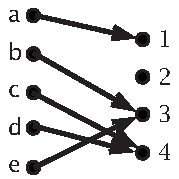
\includegraphics{images/arrowdiageg.pdf}
\end{center}
Notice that:
\begin{enumerate}
\item There is exactly one arrow coming out of each element of~$A$. This is true for the arrow diagram of any function.
\item There can be any number of arrows coming into each element of~$B$ (perhaps none, perhaps one, or perhaps many). The elements of~$B$ that do have arrows into them are precisely the elements of the range of~$f$. In this example, the range of~$f$ is $\{1,3,4\}$.
\end{enumerate}


\subsection*{Official Definition of Functions}

The preceding section provided some intuition about how and why functions are represented as sets of ordered pairs, and since ordered pairs are elements created by a Cartesian product, we learned how to view a function from $A$ to $B$ as a particular subset of $A \times B$.  This view leads to our official definition of a function:\index{Function!formal definition}

\begin{defn}{}
 Suppose $A$ and~$B$ are sets.

A set~$f$ is a 
\bfii{ function from~$A$ to~$B$} if
\begin{enumerate}[(a)]
\item \label{FunctionDefn-func-pair}
$f \subset A \times B$
\item \label{FunctionDefn-func-unique}
$\forall a \in A, \exists \mbox{ a unique } b \in B \mbox{ s.t. } (a, b) \in f$
\end{enumerate}

\noindent
(Condition (b) can also be stated as follows: every $a \in A$ is in one and only one ordered pair in $f$).  

We write ``$f \colon A \to B$" to denote that $f$ is a function from~$A$ to~$B$.
We also call
$A$  the \terminology{domain}\index{Domain!of a function} of~$f$, and
$B$ the \terminology{codomain}\index{Codomain!of a function} of~$f$.

If the pair $(a, b) \in f$, then we say that $b$ is the \terminology{image}\index{image!of an element under a function} of $a$ under the function $f$.


\end{defn}

\begin{notation}{} \label{FunctionNotation}
 Suppose $f \colon A \to B$. 
\begin{enumerate}
\item For $a \in A$, it is convenient to have a name for the element~$b$ of~$B$, such that $(a,b) \in f$. The name we use is $f(a)$:
\begin{center}
$f(a) = b$ if and only if $(a,b) \in f$.
\end{center}
\item \label{FunctionNotation-range}
 Each element~$a$ of~$A$ provides us with an element $f(a)$ of~$B$. The \terminology{range} of~$f$ is the set that includes all of these elements $f(a)$. That is,

\[ \mbox{Range of }f = \{b \in B \mbox{ such that } \exists a \in A \mbox{ with } f(a)=b.\]

The range is always a subset of the codomain. The range can be denoted $\{\, f(a) \mid a \in A \, \}$.
\end{enumerate}
\end{notation}

\begin{example}
Suppose that the function $f$ is defined by $f(x)=x^2$, on the domain $\{0,1,2,4\}$.  Then
\begin{enumerate}
\item to represent $f$ as a set of ordered pairs, each element of the domain must appear exactly once as a first coordinate, with the corresponding output given in the second coordinate.  Since there are four elements in the domain, there will be four ordered pairs: $\{(0,0), (1,1), (2,4), (4,16)\}$;
\item to give a table for $f$, we include one row for every element of the domain.  The table will be:
\begin{center}
\begin{tabular}{|c|c|}
\noalign{\hrule}
$n$ & $f(n)$ \\
\noalign{\hrule}
0 & 0 \\
 1 & 1 \\
 2  & 4 \\
 4 & 16 \\
\noalign{\hrule}
\end{tabular}
\end{center}
\item if we are asked what is $f(3)$, the answer is that $f(3)$ is \emph{undefined}, because 3 is not in the domain of $f$.  Even though we know that $3^2=9$, the formula we gave for $f$ only applies to elements that are in the domain of $f$! It is not true that $f(3)=9$;
\item the range of $f$ is the set of possible outputs: in this case, $\{0,1,4,16\}$;
\item if we are asked what is $f(2)$, the answer is $f(2)=4$;
\item is $f$ a function from $\{n \in \mathbb{N} \mid n \le 4\}$ to $\{0,1,4,16\}$?  The answer is no, because the first set is $\{0,1,2,3,4\}$, which includes the value $3$, but $3$ is not in the domain of $f$.
\item is $f$ a function from $\{0,1,2,4\}$ to $\{ n \in \mathbb{N} \mid n \le 16\}$?  The answer is yes; even though the second set has many values that are not in the range, it is a possible codomain for $f$.  A codomain can be any set that contains all of the elements of the range.
\end{enumerate}
\end{example}


\begin{exercise} \ 
 The following table describes a certain function~$g$.
\begin{center}
\begin{tabular}{|c|c|}
\noalign{\hrule}
$n$ & $g(n)$ \\
\noalign{\hrule}
2 & 7 \\
 4 & 9 \\
 6  & 11 \\
 8 & 13 \\
 10 & 15 \\
\noalign{\hrule}
\end{tabular}
\end{center}
\begin{enumerate}[(a)]
\item   \label{FunctionsChapExers-gTable-domain}
What is the domain of~$g$?
\item   \label{FunctionsChapExers-gTable-range}
What is the range of~$g$?
\item  \label{FunctionsChapExers-gTable-g(6)}
What is $g(6)$?
\item  \label{FunctionsChapExers-gTable-g(7)}
What is $g(7)$?
%\item Draw a graph to depict~$f$.
\item  \label{FunctionsChapExers-gTable-pairs}
Represent~$g$ as a set of ordered pairs.
\item  \label{FunctionsChapExers-gTable-arrow}
Draw an arrow diagram to represent~$g$.
\item  \label{FunctionsChapExers-gTable-formula}
Write down a formula that describes~$g$. 
\\(Express
$g(n)$ in terms of~$n$.)
\end{enumerate}
\end{exercise}

\begin{exercise}
 Suppose 
\begin{itemize}
\item $f$ is a function whose domain is $\{0,2,4,6\}$, 
and 
\item $f(x) = 4x - 5$, for every~$x$ in the domain. 
\end{itemize}
Describe the function in each of the following ways:
 \begin{enumerate}[(a)]
\item  \label{FunctionsChapExers-fFormula-table}
Make a table.
\item  \label{FunctionsChapExers-fFormula-pairs}
Use ordered pairs.
\item  \label{FunctionsChapExers-fFormula-arrow}
Draw an arrow diagram involving two sets.
\end{enumerate}
\end{exercise}

\begin{exercise}
 Which of the following sets of ordered pairs are functions from
$\{\var{x}, \var{y}, \var{z}\}$ to $\{\var{a},\var{b},\var{c},\var{d},\var{e}\}$? 
\begin{itemize}
\item If it is such a function, then what is its range? 
\item If it is not such a function, then explain why not.
\end{itemize}
\begin{enumerate}[(a)]
\item \label{FunctionsChapExers-Whichxy-yaxbyc}
$\{(\var{y}, \var{a}), (\var{x}, \var{b}), (\var{y},\var{c})\}$
\item \label{FunctionsChapExers-Whichxy-yaxbzc}
$\{(\var{y}, \var{a}), (\var{x},\var{b}), (\var{z},\var{c})\}$
\item \label{FunctionsChapExers-Whichxy-yaxcza}
$\{(\var{y}, \var{a}), (\var{x},\var{c}), (\var{z},\var{a})\}$
\end{enumerate}
\end{exercise}

\begin{exercise}
 Which of the following are functions from
$\{1, 2, 3\}$ to $\{\var{w},\var{h},\var{o}\}$?
(If it is not such a function, then explain why not.)
\begin{enumerate}[(a)]
\item \label{FunctionsChapExers-Which123-1w1h1o}
$\{(1, \var{w}), (1, \var{h}), (1,\var{o})\}$
\item \label{FunctionsChapExers-Which123-1h2h3h}
$\{(1, \var{h}), (2,\var{h}), (3,\var{h})\}$
\item \label{FunctionsChapExers-Which123-1h2o3w}
$\{(1, \var{h}), (2,\var{o}), (3,\var{w})\}$
\item \label{FunctionsChapExers-Which123-w1h2o3}
$\{(\var{w},1), (\var{h},2), (\var{o},3)\}$
\end{enumerate}
\end{exercise}

\begin{exercise}
 For the given sets $A$ and~$B$:
\begin{enumerate}[i] 
\item Write each function from~$A$ to~$B$ as a set of ordered pairs. (It turns out that if $|A| = m$
and $|B| = n$, then the number of functions from~$A$ to~$B$ is~$n^m$. Do you see why?)
\item Find the range of each function.
\end{enumerate}
\begin{enumerate}[(a)]
\item \label{FunctionsChapExers-FindAll-abc,d}
$A = \{\var{a},\var{b},\var{c}\}$, $B = \{\var{d}\}$
\item \label{FunctionsChapExers-FindAll-ab,cd}
$A = \{\var{a},\var{b}\}$, $B = \{\var{c},\var{d}\}$
\item \label{FunctionsChapExers-FindAll-a,bcd}
$A = \{\var{a}\}$, $B = \{\var{b},\var{c},\var{d}\}$
\item \label{FunctionsChapExers-FindAll-ab,cde}
$A = \{\var{a},\var{b}\}$, $B = \{\var{c},\var{d},\var{e}\}$
%\item $A = \{\var{a},\var{b},\var{c}\}$, $B = \{\var{d},\var{e}\}$
\end{enumerate}
\end{exercise}

\subsection*{Summary of basic function concepts}
\begin{itemize}
\item A function accepts inputs, and provides a single output for each input.
\item The set of allowable inputs is called the domain of the function.
\item Some ways of representing functions are:
\begin{itemize}
\item a formula;
\item a table;
\item a set of ordered pairs;
\item an arrow diagram.
\end{itemize}
\item Important definitions:
\begin{itemize}
\item function
\item domain
\item codomain, range
\end{itemize}
\item Notation: 
\begin{itemize}
\item $f \colon A \to B$
\item $f(a)$
\item $\{\, f(a) \mid a \in A \,\}$
\end{itemize}
\end{itemize}
%\item well-defined???


\section{One-to-One Functions}

\subsection*{Concept and definition}

\medskip\noindent
We begin this chapter with an example.

\begin{example} 
\begin{itemize}
\item Suppose Inspector Gadget knows two facts:
\begin{enumerate}
\item Alice is the thief's wife,
and
\item Alice is Bob's wife.
\end{enumerate}
Then the Inspector can arrest Bob for theft,
because a woman cannot (legally) be the wife of more than one husband.

\item On the other hand, suppose the Inspector knows:
\begin{enumerate}
\item Alice is the forger's mother,
and
\item Alice is Charlie's mother.
\end{enumerate}
Then the Inspector does not know enough to be sure who the forger is,
because it could be some other child of Alice.
\end{itemize}
This example illustrates a fundamental difference between the $\var{wife}$ function and the $\var{mother}$ function: two different people can have the same mother, but only one person can have any particular person as their wife. 
In mathematical terms, this important property of the $\var{wife}$ function is expressed by saying that the $\var{wife}$ function is ``one-to-one."
\footnote{Some math terms use the word ``injective" instead of ``one-to-one": the two are synonymous.}\index{Function!One-to-One}\index{One-to-one!informal definition}\index{Injective!also see one-to-one}
\end{example}

\begin{example}
Now let's revisit the function we saw in Example~\ref{example:functions:nonnumfuncs} part (1).  $\var{Temp}$ is the function from the set of points on the earth to the set of measured temperatures at those points.  Is $\var{Temp}$ a one-to-one function?  Not at all: it is very likely that at any given time, at least two points on earth have the same temperature.  
\footnote{It's not only likely: it's a sure thing. This can be proven mathematically, given that $\var{Temp}$ is a continuous function.  Can you prove it?}

Another way to say this is that at any given time, 

\begin{center}
there exists a temperature $b$ for which we can find two points on earth $x$ and $y$ such that  $\var{Temp}(x) = \var{Temp}(y) = b$.
\end{center}
\end{example}

\begin{exercise}
Is the function $\var{Atomic Number}$ from the set of chemical elements to the set of natural numbers a one-to-one function?  Explain why or why not.
\end{exercise}

\begin{rem}
If you have an arrow diagram of a function, then it is easy to tell whether or not the function is one-to-one. For example:

\begin{enumerate}
\item The function~$f$ of \ref{arrow11}(a) on page~\pageref{arrow11} is \emph{not} one-to-one. This is because the arrow from~$\var{b}$ and the arrow from~$\var{c}$ go to the same place, so $f(\var{b}) = f(\var{c})$. In general, if arrows from two different elements of the domain go to the same element of the range, then the function is not one-to-one. 
\item The function~$g$ of \ref{arrow11}(b) is one-to-one. This is because the arrows from two different elements of the domain never go to the same element of the range.  In short, there is only \emph{one} element of the domain that goes \emph{to} any \emph{one} element of the range.  
%(This is the reason for the terminology ``one-to-one." A function is ``two-to-one" if there are two elements of the domain mapping to each element of the range, as is true of the function~$h$ in \cref{arrow11}(c).)
\end{enumerate}
\end{rem}
%\begin{center}
\begin{figure}[h]
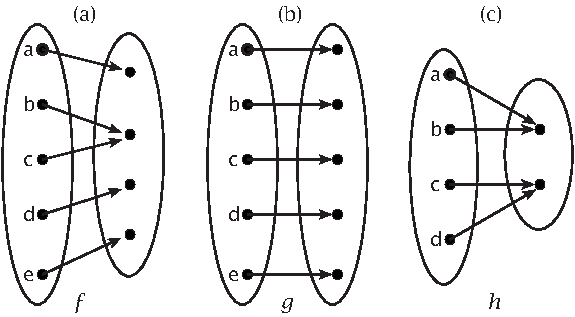
\includegraphics{images/arrow11.pdf}
\caption{Arrow diagrams of three functions $f$, $g$, and~$h$.}
\label{arrow11}
\end{figure}
%\end{center}

\begin{exercise}
Is function~$h$ of Figure \ref{arrow11} one-to-one?  Explain why or why not.
\end{exercise}

This concept of one-to-one is very useful.  If we know $A$ is a function, we know that every input of $A$ has exactly one output.  But if we know that $A$ is a one-to-one function, then we also know that every output in the range of $A$ is caused by \textbf{exactly} one input.  This notion is formalized in the following definition:

\begin{defn} \label{121defn}
Suppose $f \colon A \to B$. We say $f$ is a \bfii{ one-to-one function} iff for all $a_1,a_2 \in A$, such that
$f(a_1) = f(a_2)$, we have $a_1 = a_2$. \index{One-to-one!formal definition}
\end{defn}

\begin{exercise}\label{exercise:functions:11Exers-pairs}
 
 Each of the following sets of ordered pairs is a function from $\{1,2,3,4\}$ to $\{\var{a},\var{b},\var{c},\var{d},\var{e}\}$. Either prove that the function is one-to-one, or prove that it is not.
\begin{enumerate}[(a)]
\item  \label{11Exers-pairs-f}
$f = \{ (1,\var{a}), (2,\var{b}), (3,\var{d}), (4,\var{e})\}$
\item  \label{11Exers-pairs-g}
$g = \{ (1,\var{c}), (2,\var{d}), (3,\var{d}), (4,\var{e})\}$
\item  \label{11Exers-pairs-h}
$h = \{ (1,\var{e}), (2,\var{d}), (3,\var{c}), (4,\var{b})\}$
\item  \label{11Exers-pairs-i}
$i = \{ (1,\var{e}), (2,\var{e}), (3,\var{e}), (4,\var{e})\}$
\item  \label{11Exers-pairs-j}
$j = \{ (1,\var{a}), (2,\var{c}), (3,\var{e}), (4,\var{c})\}$
\item  \label{11Exers-pairs-k}
$k = \{ (1,\var{a}), (2,\var{c}), (3,\var{e}), (4,\var{d})\}$
\end{enumerate}
\end{exercise}

\subsection*{Proving that a function is one-to-one}

The concept of one-to-one will be very important in this course, and one of the tools we will need is the ability to prove that a function is one-to-one.  Though many of the functions we will encounter throughout this book are not algebraic, we will learn this style of proof using algebraic functions, as they are a bit easier to deal with.  Here are some examples of this type of proof. 

\begin{example}\label{example:functions:1_to_1_or_not}
Determine which of the following functions are one-to-one.  If so, give a proof.  If not, give a counterexample.
\begin{enumerate}
\item $f\colon \mathbb{R} \to \mathbb{R}$, defined by $f(x)=x +1$.

This is one-to-one.  The arc of this proof comes directly from the definition of a one-to-one function.  I need to pick two different general numbers $x$ and $y$, set their images equal to each other, and show that in actuality $x = y$.  

\noindent
So, for any real numbers $x$ and $y$, $f(x)=f(y)$ means that $x+1=y+1$.  Subtracting 1 from both sides of the equation, we conclude that $x=y$ whenever $f(x)=f(y)$.  Hence, $f$ is one-to-one.

\item $g\colon \mathbb{R} \to \mathbb{R}$, defined by $g(x)= |x|$.

This is not one-to-one.  We demonstrate this by finding two distinct real numbers whose image is the same: 
$$g(1)=|1|=1=|-1|=g(-1) ,$$
 but $1\neq -1$.  This shows that $g$ is \emph{not} one-to-one.

\item $f\colon \{1,2,3\} \to \{\var{a}, \var{b},\var{c}\}$ defined by $f=\{(1,b),(2,a),(3,a)\}$.

This is not one-to-one.  We demonstrate this by finding two distinct values in $\{1,2,3\}$ whose image is the same: 
$$f(2)=a=f(3),$$
but $2 \neq 3$.  This shows that $f$ is \emph{not} one-to-one. 

\item $h\colon \mathbb{N} \to \mathbb{N}$, defined by $h(x)=|x|$.

This is one-to-one.  Since all natural numbers are nonnegative, we have $|x|=x$ for every natural number~$x$.  So if $h(x)=h(y)$, then 
$$x = |x| = h(x)=h(y) = |y|=y,$$
making $x=y$.  Hence $h$ is one-to-one.


\end{enumerate}
\end{example}

\begin{rem}\label{rem:onetoone}
In your college algebra and calculus classes you may have used the \textbf{\emph{horizontal line test}} to get an idea of whether a function was one-to-one.  For instance, consider the function $f(x)=x +1$ from Part 1 of Example~\ref{example:functions:1_to_1_or_not} above.  Figure~\ref{fig:xplus1} is the graph of $f$ with a horizontal line passing through the function at a particular point.\index{Horizontal line test}\index{One-to-one!horizontal line test}
\begin{figure}[h]
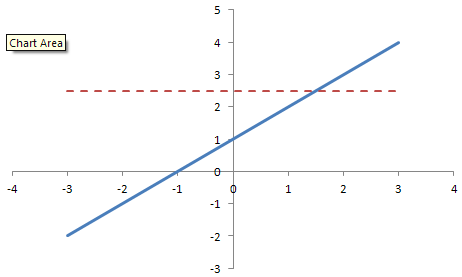
\includegraphics[width=3.5in]{images/xplus1.png}
\caption{Graph of function $f(x)=x +1$.}
\label{fig:xplus1}
\end{figure}

Based on the horizontal line test, would $f$ be a one-to-one function?  Indeed it seems so, because as we move the horizontal line up and down, it always passes through at most one point.  But how do we know somewhere outside the range of the graph we don't have a $y$-value in which the horizontal line intersects the graph at more than one point?  To prove there isn't such a $y$-value, we would need either an infinite graph, or an infinite number of graphs to view our infinite domain and range; neither of which is possible.  If you remember, in the Modular Arithmetic chapter we had this same problem for using addition and multiplication tables to prove that ${\mathbb Z}_n$ is closed for all $n \in {\mathbb N}$.   

So while the horizontal line test \emph{suggests} that $f$ is one-to-one, we would still need the proof in Part 1 of Example~\ref{example:functions:1_to_1_or_not} to \emph{prove} that it is.

On the other hand, to disprove a function is one-to-one, you only need a single counterexample.  Consider the function $g(x)= |x|$ from Part 2 of Example~\ref{example:functions:1_to_1_or_not}, which is graphed in Figure~\ref{fig:absx}.
\begin{figure}[h]
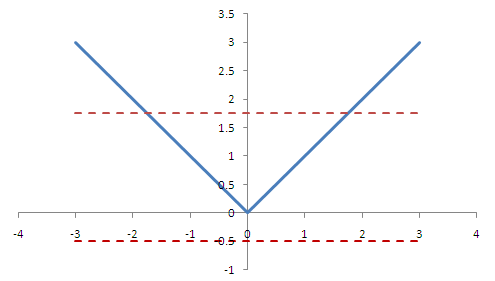
\includegraphics[width=3.5in]{images/absx.png}
\caption{Graph of function $f(x)=|x|$.}
\label{fig:absx}
\end{figure}

Using the graph we can easily identify two values in the domain that produce the same value in the codomain.  However, while the horizontal line test here suggests our counterexample, we still need to verify that the counterexample works.  So again we need the disproof in Part 2 of Example~\ref{example:functions:1_to_1_or_not}, not just a picture.

In summary, the horizontal line test can only \emph{suggest} whether a function is one-to-one or not; you still need proof or disproof.  Furthermore, the horizontal line test is usually only a good tool for functions whose domain and codomain are ${\mathbb R}$ (or subsets of ${\mathbb R}$).
\end{rem}    

% CPT I took out the following sentence, it seems repetitive.
%These examples demonstrate the general pattern of how we prove whether or not a function is one-to-one.  To prove that a function $f\colon A \to B$ \emph{is} one-to-one, we need to demonstrate that for \emph{every} $a_1, a_2 \in A$, if $f(a_1)=f(a_2)$ then we must have $a_1=a_2$.  To prove that a function $f\colon A \to B$ is \emph{not} one-to-one, we need only find a single pair of values $a_1, a_2 \in A$, for which $f(a_1)=f(a_2)$ but $a_1 \neq a_2$.  

\begin{exercise}\label{exercise:functions:11Exers}

 Each formula defines a function from~$\mathbb{R}$ to~$\mathbb{R}$. Either prove the function is one-to-one, or prove that it is not.
 \begin{enumerate}[(a)]
\item \label{11Exers-formula-f}
$f(x) = 1$.
\item \label{11Exers-formula-g}
$g(x) = x$.
\item \label{11Exers-formula-h}
$h(x) = x^2$.
\item \label{11Exers-formula-i}
$i(x) = 3x + 2$.
\item \label{11Exers-formula-j}
$j(x) = 1/ \bigl( |x| + 1 \bigr)$.
\end{enumerate}
\end{exercise}



There is an equivalent way to show functions are one-to-one that is also useful.  To see it, recall the $\var{wife}$ function from the beginning of the section.  The $\var{wife}$ function is one-to-one because one woman can't be (legally) married to two different husbands. We can express the same thing in a different way by saying that two different husbands must be married to two different wives. These two statements are \bfii{ contrapositives}\index{contrapositive} of each other, and are in fact equivalent.  (``contrapositive'' is a logical term--you may have run across it before in a Discrete Math class.)
 
If we generalize this reasoning to arbitrary one-to-one functions, we have the following two equivalent statements:
\begin{itemize}
\item
A function is one-to-one iff any element of the range is mapped from only one element of the domain;
\item
A function is one-to-one iff two different elements of the domain always map to two different elements of the range.
\end{itemize}

We formalize this equivalence in the following alternative definition of one-to-one:

\begin{defn} \label{121defn2}\emph{(Alternate)}
Suppose $f \colon A \to B$. We say $f$ is a \bfii{ one-to-one function}\index{One-to-one!alternate definition} iff for all $a_1,a_2 \in A$, such that $a_1 \neq a_2$, we have $f(a_1) \neq f(a_2)$. 
\end{defn}

% \begin{prop}\label{proposition:functions:alternate121defn} \emph{(Alternate characterization of one-to-one functions)} 

% A function $f \colon A \to B$ is one-to-one if and only if \index{One-to-one!contrapositive based definition}
% \medskip

% $ \forall a_1,a_2 \in A, \bigl( a_1 \neq a_2 \implies f(a_1) \neq f(a_2) \bigr)$.
% \medskip 
% \noindent
 % The notation $\forall a_1, a_2 \in A$ is short for $\forall a_1\in A, \forall a_2 \in A$.
 % \end{prop}
 
% Notice that the proposition contains an "if and only if" clause.  This means that we have to prove the statement in both directions, i.e. 

% \begin{center}
% If a function $f\colon A \to B$ is one-to-one, then $$\forall a_1, a_2 \in A, \bigl( a_1 \neq a_2 \eif f(a_1) \neq f(a_2)\bigr).$$
% \end{center}

% and

% \begin{center}
% If $\forall a_1, a_2 \in A, \bigl( a_1 \neq a_2 \eif f(a_1) \neq f(a_2)\bigr)$, then $f\colon A \to B$ is one-to-one.
% \end{center}

% We will prove the first direction, and the second will be a fill-in-the-blank exercise.

% \begin{proof} 
% Let $f \colon A \to B$ be one-to-one. Given $a_1,a_2 \in A$, we know, from the definition of one-to-one,  that
	% \[  f(a_1) = f(a_2) \eif a_1 = a_2 . \]
% So the contrapositive of this implication is also true. That is,
	% \[ a_1 \neq a_2 \eif f(a_1) \neq f(a_2) . \]
% \end{proof}

% \begin{exercise}
% Prove the second direction of Proposition~\ref{proposition:functions:alternate121defn}
% \begin{enumerate}[(a)]
% \item
% Let's assume $\forall a_1, a_2 \in A, \bigl( a_1 \neq a_2 \eif f(a_1) \neq f(a_2)\bigr) $.  Then if $f(a_1) = f(a_2)$, by the \_\_\_\_\_\_\_\_\_\_\_\_\_\_\_ of our assumption it follows that \_\_\_\_\_\_\_\_\_\_\_\_\_\_\_\_.
% \item
% Hence $f(a_1) = f(a_2) \eif a_1 = a_2$, and therefore by Definition \ref{121defn}, \_\_\_\_\_\_\_\_\_\_\_\_\_\_\_\_\_\_\_\_.
% \end{enumerate}
% \end{exercise}
 
%\begin{prop}
%Let $f \colon \real\to \real$ be defined by $f(x)=x/2 + 1$.  Then $f$ is one-to-one.
%\end{prop}

%In some cases, when a function is not one-to-one, it is easy to find examples of distinct elements whose images are equal.  In other cases, such examples may be hard to find.
When you don't know whether or not a particular function is one-to-one, a good strategy is to try to prove that it's one-to-one.  If the proof works, great! -- we are done.  If the proof fails, the manner in which it fails may indicate an example to show that the function is not one-to-one.  Here is an example of this technique.

\begin{example}
Let $f\colon \mathbb{N} \to \mathbb{N}$ be defined by $f(n)=(n-2)^2 + 1$.  Is $f$ one-to-one?
\medskip

First let's try to prove that $f$ is one-to-one.   
Start with arbitrary elements $m, n \in \mathbb{N}$, and suppose that $f(m)=f(n)$.  By the definition of $f$, this means that $(m-2)^2 + 1=(n-2)^2 + 1$, or $(m-2)^2 =(n-2)^2 $.  Two numbers have the same square, if and only if they are equal in absolute value, so it follows that $m-2 = \pm (n-2)$.  There are now two cases:
\begin{itemize}
\item
If $m-2=+(n-2)$ then adding 1 to each side, we get $m=n$.  
\item
If $m-2 = -(n-2) = -n+2$, then adding 1 to each side, we get $m=-n+4$.  
\end{itemize}
Since $m,n \in \mathbb{N},$ it's not hard to see that if $n \ge 4$, then $-n+4$ is not a natural number.  But if $n$ is 1,2,3 then $-n+4 \in \mathbb{N}$. For example $n=1$ gives $m = 3$, which suggests that $f(1) = f(3)$. We may indeed check that  $f(1) = f(3)$. 

Now the great thing about cases where $f$ is not one-to-one is, the writeup of the solution is very simple. All you have to do is give one example of two different values that return the same function value. In the current example we have: 
% So we look at these three cases:
% \begin{itemize}
% \item
% If $n=1$ then $m=-n+2=1=n$, so this case is not a problem.  
% \item
% But if $m=2$ and $n=0$, then $(m-1)^2=1^2=(-1)^2=(n-1)^2$, so $f(m)=f(n)$ even though $m \neq n$.  (We could also choose $m=0$ and $n=2$.)  This is the example that shows that $f$ is not one-to-one.
% \end{itemize}
% \end{scratchwork}

\noindent
\begin{solution}
$f$ is \emph{not} one-to-one because $f(1) = 2$ and $f(3) = 2$. 
% To prove this, let $m = 0$ and $n = 2$. Then 
	% $$ f(m) = f(0) = (0-1)^2 = 1$$
% and
	% $$ f(n) = f(2) = (2-1)^2 = 1 ,$$
% so $f(m) = f(n)$. On the other hand, we also have $m = 0 \neq 2 = n$, so $m \neq n$. Since $f(m) = f(n)$ and $m \neq n$, we know that $f$ is not one-to-one.
\end{solution}

\noindent  
So the writeup is easy: two values is all it takes. The hard thing is finding the two values!
\end{example}

\begin{exercise} 
For each function, either prove that it is one-to-one, or prove that it is not.
\begin{enumerate}[(a)]
\item \label{IsIt11?-linear}
 $f \colon \rational \to \rational$ defined by $f(x)=3x/5 - 2$.
\item \label{IsIt11?-square}
 $f \colon {\mathbb N} \to {\mathbb N}$ defined by $f(x)=x^2$.
\item \label{IsIt11?-abs}
 $g \colon \real \to \real$ defined by $g(x)= \left|(x+1)/2 \right|$.
\item \label{modular}
 $g \colon {\mathbb Z}_6 \to {\mathbb Z}_6$ defined by $g(x)= x \oplus 2$ .
\item \label{modular_m}
 $g \colon {\mathbb Z}_8 \to {\mathbb Z}_8$ defined by $g(x) = x \odot 2 $ .
\item \label{modular_m}
 $g \colon {\mathbb Z}_{11} \to {\mathbb Z}_{11}$ defined by $g(x) =  x \odot 2$ .
\item 
 $g \colon {\mathbb Z}_7 \to {\mathbb Z}_7$ defined by $g(x)= x \odot x$ .
\item 
 $g \colon {\mathbb Z}_8 \to {\mathbb Z}_8$ defined by $g(x)= x \odot x \odot x$ .
\item 
 $g \colon {\mathbb Z}_7 \to {\mathbb Z}_7$ defined by $g(x)= x \odot x \odot x$ .
\item
 $g \colon {\mathbb C}\setminus \{0\}  \to {\mathbb C}\setminus \{0\} $ defined by $g(z) =  z^{-1}$ .
 \end{enumerate}
\end{exercise}

%\begin{rem}[(alternative terminology)]
%Many mathematicians use the word ``\emph{injective}," rather than ``one-to-one." (This comes from French.) Also, a function that is one-to-one can be called an \emph{injection}.
%\end{rem}

%\subsection*{Summary of one-to-one}
%\item Important definitions:
%\begin{itemize}
%\item one-to-one
%\end{itemize}
%\item Notation:
%\begin{itemize}
%\item $\forall a_1, a_2 \in A$ means $\forall a_1 \in A, \forall a_2 \in A$.
%\end{itemize}
%\end{summary}

\section{Onto Functions}

\subsection*{Concept and definition}
In an arrow diagram of a function $f \colon A \to B$, the definition of a function requires that there is exactly one arrow out of each element of~$A$,  but it says nothing about the number of arrows into each element of~$B$. There may be elements of~$B$ with lots of arrows into them (unless the function is one-to-one), and there may be other elements of~$B$ that have no arrows into them. 
The function is called ``onto"\index{Onto}\index{Surjective!also see onto}\index{Function!onto}
\footnote{Some math terms use the word ``surjective" instead of ``onto": the two are synonymous.}
 if all of the elements of~$B$ are hit by arrows; none are missed.

\begin{example}
Figure \ref{arrowontofig} shows arrow diagrams of various functions, some onto and some not.
\end{example}

\begin{center}
\begin{figure}[h]
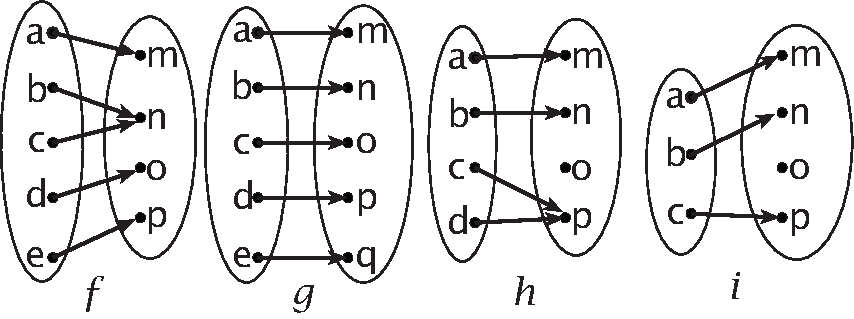
\includegraphics[scale=0.6]{images/arrowonto.pdf}
\caption{Arrow diagrams for various functions}
\label{arrowontofig}
\end{figure}
\end{center}

In Figure~\ref{arrowontofig},
\begin{itemize}
\item
$f$ is onto, but not one-to-one. 
\item
$g$ is both one-to-one and onto. 
\item
$h$ is neither one-to-one nor onto. 
\item
$i$ is one-to-one, but not onto.
\end{itemize}

\begin{example}
 Not every woman is a mother. 
%This means there is some woman~$w$, such that there does \emph{not} exist any person~$p$, such that $\var{mother}(p) = w$. 
This means that if you draw an arrow from each person to his or her mother, there will be some women who have no arrows into them. So the function 
\[ \var{mother} \colon \var{People} \to \var{Women} \]
 is \emph{not} onto.
\end{example}

\begin{exercise}
Is the function $\var{Atomic Number} \colon \{ \mbox{ Chemical Elements } \} \to \mathbb{N}$ onto?  Explain why or why not.
\end{exercise}

The following is the "official" definition  of onto.

\begin{defn}
Suppose $f \colon A \to B$. We say $f$ is \bfii{ onto} if for all $b \in B$, \index{Onto!formal definition}
there is some $a \in A$, such that $f(a) = b$. 
\end{defn}

In words: if I pick any value in the codomain of $f$, there is some value in the domain that produces it.

\begin{exercise}
If the function $f$ is onto, then what is the relation between the range of $f$ and the codomain of $f$? \emph{(Hint: can there be any elements in the codomain that are not in the range?).}
\end{exercise}


\subsection*{Proving that a function is onto}

The following examples show how to prove that a function is onto.

\begin{example}\label{example:functions:onto}
\begin{itemize}
\item
 Consider the  function:

$f\colon \mathbb{R} \to \mathbb{R}$ defined by $f(x)=x +1$.

Recall that a function is onto if for every value in the codomain, there is a value in the domain that produces it.  
So pick an arbitrary value in the codomain $\mathbb{R}$ and call it $y$.  By the definition of our function $f$, $f(x)=y$ means that $x+1=y$.  Solving for $x$ gives $x = y - 1$.  Now $x$ is also a real number (by  closure of $\mathbb{R}$ under $-$): so we have found an $x$ in the domain of $f$ such that  $f(x) = y$.  Therefore $f$ is onto.

\item 
Consider the function 
$h\colon \mathbb{N} \to \mathbb{N}$, defined by $h(x)=|x|$.

Since all natural numbers are nonnegative, we have $h(x)=|x|=x$ for every natural number $x$.  So for an arbitrary value $y$ in the codomain $\mathbb{N}$, we have $h(y) = y$ (note $y$ is also in the domain of $h$). Therefore $h$ is onto.
\end{itemize}

\end{example}

It is typically easier to prove that a function is \emph{not} onto. All you have to do is provide a counterexample:

\begin{example}\label{example:functions:not_onto} 
\begin{itemize}
\item
Consider the function $f\colon \{1,2,3\} \to \{\var{a}, \var{b},\var{c}\}$ defined by $f=\{(1,\var{b}),(2,\var{a}),(3,\var{a})\}$.
Notice that $c$ never appears as an image in this function.  This shows that $f$ is not onto. 
\item
Consider the function $g\colon \mathbb{R} \to \mathbb{R}$ defined by $g(x)= |x|$. To show that $g$ is not onto, we only need to find a single number $y$ in the codomain that  is not mapped onto.  $y=-1$ is one example: we can never have $|x|=-1$ for any real number $x$.  This shows that $g$ is not onto.
\item
Consider the function $h\colon \mathbb{Z}_5 \to \mathbb{Z}_5$ defined by $h(x)= x \odot x $. We may list the values of $h(x)$ for $x = 0,1,2,3,4$: they are $0,1,4,4,1$ respectively. There is no $x$ such that $h(x) = 3$, so $h$ is not onto.
\end{itemize}
\end{example}


% CPT I think this is redundant
% In summary then, to prove that a function $f \colon A \to B$ is onto, we wish to show:
 %$$\forall b \in B, \exists a \in A \mbox{ s.t. } f(a) = b$$
% 
%So first we choose a general element $b$ of the codomain, and then we use the definition of the function to determine a way to define a general element $a$ in the domain such that $f(a) = b$.  Since $b$ is general , this defining of $a$ works for all $b$.  And therefore the function is onto.
%
%As always, if the function is not onto, you only need to show a counterexample that shows this.

Since ``onto'' proofs require working backwards, sometimes some preliminary scratchwork is required before writing out the actual proof.

\begin{example}
Define $g \colon \mathbb{R} \to \mathbb{R}$ by $g(x) = 5x - 2$. Show $g$ is onto.


\begin{scratchwork}
Just as in the previous examples, given any $y \in \mathbb{R}$  we need to find a value of~$x$ that makes $g(x) = y$. So we start with the equation $g(x) = y$ and solve for $x$:
\begin{align*}
g(x) &= y \\
5x-2 &= y \\
5x &= y + 2 \\
x &= \frac{y+2}{5}
\end{align*}

\noindent
Now that we have $x$, lets do our proof.
\end{scratchwork}

\begin{proof} 
Given $y \in \mathbb{R}$, let $x = (y+2)/5$.  Since the reals are closed under addition and non-zero division, it follows that $x \in \mathbb{R}$. Then
\[ g(x) = 5x - 2 = 5 \left( \frac{y+2}{5} \right) - 2 = (y+2) - 2 = y . \]
Therefore $g$ is onto.
\end{proof}

\medskip
Although you need the scratchwork to come up with the formula for $x$, you don't need to include the scratchwork in your proof. It's actually much cleaner without it.
\end{example}

%\begin{rem}
%Some ``onto'' proofs are a bit more complicated than what is described above, because it may not be possible to go directly from ``Given $b \in B$'' to ``let $a = \raise 3pt \hbox{\boxit{\phantom{M}}}$.'' Sometimes it is necessary to insert calculations (or other explanations) between ``given~$b$'' and ``let~$a$.'' Some good examples of this will be seen in \cref{CompositionTheoryExers}.
%\end{rem}

%\begin{rem}[(alternative terminology)]
%Some mathematicians use the word \emph{surjective} rather than onto (this comes from French -- similarly,  \emph{injective} can replace one-to-one). A function that is onto (resp. one-to-one) can be called a \emph{surjection} (resp \emph{injection}).
%\end{rem}
% 
%\section*{Proof exercises}

\begin{rem}
In your college algebra and calculus classes you may have used the horizontal line test\index{Onto!horizontal line test}\index{Horizontal line test} to show whether a function was onto.  
For instance, recall the function $f(x)=x +1$ shown in Figure~\ref{fig:xplus1}. is the graph of $f$ with a horizontal line passing through the function at a particular point.
Based on the horizontal line test, would $f$ be a onto function? What we're looking for is whether or not each horizontal line intersects the graph in \emph{at least} one point. The figure suggests this is true, but to prove it for \emph{all} horizontal lines we would need an infinite graph.  So again, the horizontal line test \emph{suggests} that $f$ is onto, but we still need the proof in Part 1 of Example~\ref{example:functions:onto} to \emph{prove} that it is.

On the other hand, to disprove a function is onto, you only need a counterexample.  Consider the function $g(x)= |x|$ shown in Figure~\ref{fig:absx}. Using the graph, we can easily find a horizontal line that doesn't intersect the graph: this corresponds to a value in $\mathbb{R}$ that is not in the range of $g$.  But while the horizontal line test here suggests a counterexample to show $g$ is not onto, we still need to verify that it works.
\end{rem}    

  
\begin{exercise}\label{exercise:functions:OntoExers} \ 
Each formula defines a function from~$\mathbb{R}$ to~$\mathbb{R}$. Either prove that the function is onto, or prove that it is not.
\begin{enumerate}[(a)]
\item \label{OntoExers-formula-a(x)}
 $a(x) = 1$.
\item \label{OntoExers-formula-b(x)}
 $b(x) = x$.
\item \label{OntoExers-formula-c(x)}
 $c(x) = x^2$.
\item \label{OntoExers-formula-d(x)}
 $d(x) = 3x + 2$.
\item \label{OntoExers-formula-e(x)}
 $e(x) = 1/ \bigl( |x| + 1 \bigr)$.
\item \label{OntoExers-formula-f(x)}
 $f(x) = 4x - 6$.
\item \label{OntoExers-formula-g(x)}
 $g(x) = \root 3 \of {x+5} - 5$.
\end{enumerate}
\end{exercise}

\begin{exercise}\label{exercise:functions:OntoExers-pairs}
Each of the following sets of ordered pairs is a function from $\{1,2,3,4,5\}$ to $\{\clubsuit,\diamondsuit,\heartsuit,\spadesuit\}$. Either prove that the function is onto, or prove that it is not.
\begin{enumerate}[(a)]
\item \label{OntoExers-pairs-a}
$a = \{ (1,\clubsuit), (2,\diamondsuit), (3,\heartsuit), (4,\spadesuit), (5,\clubsuit) \}$
\item \label{OntoExers-pairs-b}
$b = \{ (1,\clubsuit), (2,\heartsuit), (3,\clubsuit), (4,\heartsuit), (5,\clubsuit) \}$
\item \label{OntoExers-pairs-c}
$c = \{ (1,\heartsuit), (2,\heartsuit), (3, \heartsuit), (4,\heartsuit), (5, \heartsuit) \}$
\item \label{OntoExers-pairs-d}
$d = \{ (1,\diamondsuit), (2,\spadesuit), (3, \heartsuit), (4,\spadesuit), (5, \clubsuit) \}$
\item \label{OntoExers-pairs-e}
$e = \{ (1,\clubsuit), (2,\spadesuit), (3, \heartsuit), (4,\spadesuit), (5, \clubsuit) \}$
%\item \label{OntoExers-colour}
% If $f$ is a vertex-colouring of the complete graph on $n$ vertices that uses $n$ colours, is $f$ onto?
%\emph{Justify your answer.}
\end{enumerate}
\end{exercise}


\begin{exercise}
For each of the following  functions, either prove that it is onto, or prove that it is not.
\begin{enumerate}[(a)]
\item \label{modular_m}
 $g \colon {\mathbb Z}_5 \to {\mathbb Z}_{5}$ defined by $g(x) =  (x \odot 2) \oplus 3$ .
\item 
 $g \colon {\mathbb Z}_7 \to {\mathbb Z}_7$ defined by $g(x)= (x \odot x) \oplus 1 $ .
\item 
 $g \colon {\mathbb Z}_9 \to {\mathbb Z}_9$ defined by $g(x)= x \odot x \odot x$ .
\item 
 $g \colon {\mathbb Z}_7 \to {\mathbb Z}_7$ defined by $g(x)= x \odot x \odot x$ .
\item
 $g \colon {\mathbb C}\setminus \{1\}  \to {\mathbb C}\setminus \{0\} $ defined by $g(z) =  \frac{1}{z-1}$ .
\end{enumerate}
\end{exercise}

When a function is defined \emph{piecewise}, the one-to-one and  onto proofs are a little harder:

\begin{example}\label{example:functions:piecewise}

  For instance, consider the function $f$ from~$\mathbb{R}$ to~$\mathbb{R}$ defined by:
$$ f(x) = 
\begin{cases}
e^x & \mbox{if $x > 0$} \\
1 - x^2 & \mbox{if $x \le 0$}
\end{cases} $$
If you graph this function, you wil find that the horizontal line tests suggest $f(x)$ is indeed one-to-one and onto. To complete the actual proof, we need to prove four separate statements:
\begin{enumerate}[(a)] 
\item
If $y > 1$, there exists a unique $x>0$ such that $e^x = y$ (thus $f(x)=y$).
\item
If $y \le 1$, there exists a unique $x \le 0$ such that $1-x^2 = y$ (thus $f(x)=y$).
\end{enumerate}
From these two facts, we see that $f(x)$ is onto, because for any $y$ (whether $>1$ or $\le 1$) there exists an $x$ such that $f(x)=y$. 

To show that $f(x)$ is one-to-one, we will need two additional statements:
\begin{enumerate}[(c)] 
\item
If $y > 1$, there exists no $x\le0$ such that $1 - x^2 = y$ (thus $f(x)=y$).
\item
If $y \le 1$, there exists a unique $x \le 0$ such that $1-x^2 = y$ (thus $f(x)=y$).
\end{enumerate}
From these two facts (together with (a) and (b)) we find that for any $y$ (whether $>1$ or $\le 1$) there is \emph{exactly} one $x$ such that $f(x)=y$.
\end{example}
 
\begin{exercise} \label{OntoCasesExer}
 Deine functions $f$ and~$g$ from~$\mathbb{R}$ to~$\mathbb{R}$ by:
$$ f(x) = 
\begin{cases}
1/x & \mbox{if $x > 0$} \\
x + 1 & \mbox{if $x \le 0$}
\end{cases} $$
and
$$ g(x) = 
\begin{cases}
1/x & \mbox{if $x > 0$} \\
x - 1 & \mbox{if $x \le 0$}
 . \end{cases} $$
 Show:
 \begin{enumerate}[(a)]
 \item \label{OntoCasesExer-fOnto}
 $f$ is onto;
 \item \label{OntoCasesExer-gNotOnto}
 $g$ is not onto;
 \item \label{OntoCasesExer-fNot11}
 $f$ is not one-to-one;
 and
 \item \label{OntoCasesExer-g11} 
 $g$ is one-to-one.
\end{enumerate}
\end{exercise}

%\begin{exers} \label{OntoTheoreticalExers} \ 
%\begin{enumerate}
%% \item Give an example of a function $f \colon \real \to \real$ that is both one-to-one and onto.
%% ({\em Justify your answer!\/})
%% \item Give an example of a function $f \colon \real \to \real$ that is one-to-one, but not onto.
%% ({\em Justify your answer!\/})
%% \item Give an example of a function $f \colon \real \to \real$ that is onto, but not one-to-one.
%% ({\em Justify your answer!\/})
%% \item \label{m>nIFFonto}
%% Suppose $m,n \in \mathbb{N}$. Show $m \ge n$ if and only if there exists an onto function $f \colon \{1,2,3,\ldots,m\} \to \{1,2,3,\ldots,n\}$.
%% \hint{SHOULD GIVE A HINT!!!}
%\end{enumerate}
%\end{exers}

%CPT  There are no exercises in this section, and I'm not sure that we need it at this point
%\subsection*{Image and pre-image}
%
%Given a function $f: A \rightarrow B$ and $x \in A$, we have referred to $f(x)$ as the \emph{image} of $x$. But suppose instead of considering how $f$ acts on one particular input $x \in A$, instead we consider what $f$ does to a %\emph{set} of inputs. Naturally, a set of inputs will produce a set of outputs.  The following definition formalizes this concept.
%
%\begin{defn}
%Suppose $f \colon A \to B$.
%\item For any subset $A_1$ of~$A$, the \terminology{image} of $A_1$ under~$f$ is
%$$ f(A_1) = \bigset{\vphantom{\big|} f(a) }{ a \in A_1 } .$$
%Note that  $f(A_1) \subset B$.
%\end{defn}
%
%
%\item For any subset $B_1$ of~$B$, the \define[pre-image|indsee{inverse image}]{pre-image} (or \define[inverse!image]{inverse image}) of $B_1$ under~$f$ is
%$$ f^{-1}(B_1) = \bigset{\vphantom{\big|} a \in A }{ f(a) \in B_1 } .$$
%It is a subset of~$A$. When $B_1 = \{b\}$ has only one element, we usually write $f^{-1}(b)$, instead of $f^{-1} \bigl( \{b\} \bigr)$.
%\end{enumerate}
%\end{defn}
%
%\begin{example} \ 
%\begin{enumerate}
%\item For the function $\var{mother} \colon \var{PEOPLE} \to \var{WOMEN}$, $\var{mother}^{-1}(m)$ is the set of all children of~$m$.
%\item For the function $f \colon \mathbb{R}  \to \mathbb{R}$ defined by $f(x) = x^2$:
%\begin{enumerate}
%\item We have $f^{-1}(4) = \{2,-2\}$, because $2$ and~$-2$ are all of the square roots of~$4$.
%\item We have $f^{-1} \bigl( [-4,4] \bigr) = [-2,2]$, because $-4 \le x^2 \le 4$ iff $-2 \le x \le 2$.
%\end{enumerate}
%\end{enumerate}
%\end{example}
%
%We need and arrow diagram example for image and pre-image
%
%
%\begin{warn}
%The fact that we write $f^{-1}(B_1)$ does not imply that $f^{-1}$ is a function. This is simply a notation that refers to the set we have defined.
%\end{warn}



%Here are examples of proofs involving inverse images:

%\begin{eg} \label{InvImgContainEg}
%Suppose $f \colon A \to B$ and $B_1 \subset B$.
%\begin{enumerate}
%\item \label{InvImgContainEg-f(f(B1))inB1}
% We have $f \bigl( f^{-1}(B_1) \bigr) \subset B_1$.
%\item \label{InvImgContainEg-f(f(B1))=B1}
 %If $f$ is onto, then $f \bigl( f^{-1}(B_1) \bigr) = B_1$.
%\end{enumerate}

%\begin{proof}
%\pref{InvImgContainEg-f(f(B1))inB1} Let $b \in f \bigl( f^{-1}(B_1) \bigr)$. By definition, we have
	%$$ f \bigl( f^{-1}(B_1) \bigr) = \bigset{ f(a) }{ a \in f^{-1}(B_1) } ,$$
%so we must have $b =  f(a_1)$, for some $a_1 \in f^{-1}(B_1)$. From the definition of $f^{-1}(B_1)$, we know that $f(a_1) \in B_1$. Therefore $b = f(a_1) \in B_1$. Since $b$ is an arbitrary element of $f \bigl( f^{-1}(B_1) \bigr)$, this implies that $f \bigl( f^{-1}(B_1) \bigr) \subset B_1$, as desired.

%\smallskip
%\pref{InvImgContainEg-f(f(B1))=B1} Assume $f$ is onto. We know, from~\pref{InvImgContainEg-f(f(B1))inB1}, that $f \bigl( f^{-1}(B_1) \bigr) \subset B_1$, so it suffices to show that $B_1 \subset f \bigl( f^{-1}(B_1) \bigr)$. 

%Let $b \in B_1$ be arbitrary. Because $f$ is onto, we know there exists $a_1 \in A$, such that $f(a_1) = b$. Then $f(a_1) = b \in B_1$, so $a_1 \in  f^{-1}(B_1)$. Therefore
	%$$ f(a_1) \in \bigset{ f(a) }{ a \in f^{-1}(B_1) } = f \bigl( f^{-1}(B_1) \bigr) .$$
%Since $f(a_1) = b$, we conclude that $b \in f \bigl( f^{-1}(B_1) \bigr)$.
%\end{proof}
%\end{eg}



 

%\begin{exers} \label{InverseImgEx}
%Suppose that $f \colon A \to B$, that $A_1 \subset A$, and that $B_1 \subset B$.
%\begin{enumerate}
%\item \label{InverseImgEx-f(A2)inf(A1)}
% Show that if $A_2 \subset A_1$, then $f(A_2) \subset f(A_1)$.
%\item \label{InverseImgEx-finv(B2)infinv(B1)}
 %Show that if $B_2 \subset B_1$, then $f^{-1}(B_2) \subset f^{-1}(B_1)$.
%\item \label{InverseImgEx-Ainf(f(A))}
 %Show $A_1 \subset f^{-1} \bigl( f(A_1) \bigr)$.
%\item \label{InverseImgEx-A1=}
 %Show that if $f$ is one-to-one, then $A_1 = f^{-1} \bigl( f(A_1) \bigr)$.
%\item \label{InverseImgEx-=f(A1)}
 %Show $f \Bigl( f^{-1} \bigl( f(A_1) \bigr) \Bigr) = f(A_1)$.
%\end{enumerate}
%\end{exers}


%\begin{summary}
%\item Important definitions:
%\begin{itemize}
%\item onto
%\item image, pre-image
%\end{itemize}
%\item How to prove $\forall$-statements was discussed.
%\item How to prove $\exists$-statements was discussed.
%\item Notation:
%\begin{itemize}
%\item $f(A_1)$, $f^{-1}(B_1)$
%\end{itemize}
%\end{summary}
 
 
\section{Bijections}

\subsection*{Concept and definition}

\medskip\noindent
Some ``especially nice" functions are both one-to-one and onto.

\begin{defn}
 A function is a \terminology{bijection} if and only if it is both one-to-one and onto.\index{Bijection!definition of}
\end{defn}

In words, a bijection has the following properties:
\begin{itemize}
\item
All inputs have only one output (function)
\item
All outputs are paired with only one input (one-to-one)
\item
And all possible outputs of the codomain are paired (onto)
\end{itemize}

%\begin{rem}
%You may recall that a one-to-one function may be called an ``injection," and an onto function may be called a ``surjection."  The term ``bijection" comes from having both of these properties.
%\end{rem}

 \begin{example}\label{example:functions:MarriedEg}
 Consider a hypothetical country $\var{Married}$, in which 
 \begin{itemize}
 \item everyone is married (to only one person --- there is no polygamy),
 and
 \item every marriage is between a man and a woman (there are no same-sex marriages). 
 \end{itemize}
Let $\var{Men}$ = \{men in the country\}, and 
$\var{Women}$ = \{women in the country\}.
Then $\var{wife} \colon \var{Men} \to \var{Women}$ is a bijection, since:
\begin{itemize}
 \item Two different men cannot have the same wife, so we know that $\var{wife}$ is one-to-one. 
 \item Every woman is the wife of some man (because everyone is married), so $\var{wife}$ is also onto.
 \end{itemize}
Similarly, the function $\var{husband} \colon \var{Women} \to \var{Men}$ is also a bijection.
 \end{example}

\begin{rem}
In the country $\var{Married}$ described above, it is clear that the number of men is exactly equal to the number of women. (If there were more men than women, then not every man could have a wife; if there were more women than men, then not every women could have a husband.) This is an example of the following important principle:
	
\begin{center}
If $A$ and $B$ are finite sets, and there exists a bijection from~$A$ to~$B$, 
	then $A$ and~$B$ have
	 the same number of elements.
\end{center}

Finding a bijection is one way to show two sets have the same number of elements.
\end{rem}

\begin{exercise}
Draw an arrow diagram of a bijection.
\end{exercise}

\begin{exercise}
Is the function $\var{Atomic Number} \colon \{ \mbox{ Chemical elements } \} \to \mathbb{N}$ a bijection?  Justify your answer.
\end{exercise}


\subsection*{Proving that a function is a bijection}

Since a bijection  is both one-to-one and onto, a proof that a function is a bijection (usually) has two parts:
	\begin{enumerate}
	\item Show that the function is one-to-one.
	\item Show that the function is onto.
	\end{enumerate}
The two parts can come in either order: it is perfectly acceptable to first prove that the function is onto, and then prove that it is one-to-one.

How would you show that function is not a bijection?  You guessed it, by counterexample.  You only need a counterexample that shows either the function is not onto, or is not one-to-one, because a bijection requires both.

\begin{example}\label{example:functions:5x-7BijectionEg}
Define $f \colon \mathbb{R} \to \mathbb{R}$ by $f(x) = 5x-7$. Then $f$ is a bijection.

\begin{proof}
It suffices to show that $f$ is both one-to-one and onto:
\begin{itemize}
\item  \emph{(one-to-one)} Given $x_1,x_2 \in \mathbb{R}$, such that $f(x_1) = f(x_2)$, we have
$$5x_1 - 7 = 5x_2 - 7.$$
\medskip
\noindent
Adding 7 to both sides and dividing by 5, we have
$$ \frac{(5x_1-7)+7}{5} =  \frac{(5x_2-7)+7}{5},$$
\noindent
Which implies $x_1=x_2$. So $f$ is one-to-one.
\item
\emph{(onto)}  Given $y \in \mathbb{R}$, let $x = (y+7)/5$. Then
$$ f(x) = 5x-7 = 5 \left( \frac{y+7}{5} \right) - 7 = (y+7) - 7 = y,$$
So $f$ is onto.

Since $f$ is both one-to-one and onto, we conclude that $f$ is a bijection.
\end{itemize}
\end{proof}
\end{example} 

\begin{exercise}\label{exercise:functions:BijectRtoRExer}
Each formula defines a function from~$\mathbb{R}$ to~$\mathbb{R}$.  Either prove the function is a bijection, or prove that it is not.
\begin{multicols}{2}
\begin{enumerate}[(a)]
\item \label{BijectRtoRExer-(5x+2)}
$a(x) = 5x+2$
\item \label{BijectRtoRExer-(2x-5)}
$b(x) = 2x - 5$
\item \label{BijectRtoRExer-(12x-15)}
 $c(x) = 12x-15$
\item \label{BijectRtoRExer-(-15x-12)}
$d(x) = -15x - 12$
\item \label{BijectRtoRExer-(x^3)}
$e(x) = x^3$
\item \label{BijectRtoRExer-(root3of(x-4))}
$f(x) = \root 3 \of {x-4} $
\item \label{WhichBijRExer-(1)}
$a(x) = 1$.
\item \label{WhichBijRExer-(x)}
$b(x) = x$.
\item \label{WhichBijRExer-(x^2)}
$c(x) = x^2$.
\item \label{WhichBijRExer-(3x+2)}
$d(x) = 3x + 2$.
\item \label{WhichBijRExer-(1/(|x|+1))}
$e(x) = 1/ \bigl( |x| + 1 \bigr)$.
\item \label{WhichBijRExer-(4x-6)}
$f(x) = 4x - 6$.
\item \label{WhichBijRExer-(root3ofx-5)}
$g(x) = \root 3 \of {x} - 5$.
\item \label{WhichBijRExer-(sqrt(x^2+1))}
$h(x) = \sqrt{x^2 + 1}$
\end{enumerate}
\end{multicols}
\end{exercise}
%
%\begin{exers} \label{BijectLinFracExer} \ 
%\begin{enumerate}
%\item Let 
%$$ \mbox{$A = \{\, a \in \real \mid a \neq 2 \,\}$ and $B = \{\, b \in \real \mid b \neq 3 \,\}$,} $$
%and define $f \colon A \to B$ by 
%$$f(a) = \frac{3a+1}{a-2} .$$
%Show that $f$ is a bijection.
%
%\item Let 
%$$ \mbox{$X = \{\, x \in \real \mid x \neq -1 \,\}$ and $Y = \{\, y \in \real \mid y \neq 5/2 \,\}$,} $$
%and define $g \colon X \to Y$ by 
%$$g(x) = \frac{5x-3}{x+1} .$$
%Show that $g$ is a bijection.
%\end{enumerate}
%\end{exers}



\begin{exercise}\label{exercise:functions:LinearWhenBijectionExer}
Let $a,b \in \mathbb{R}$, and define $f \colon \mathbb{R} \to \mathbb{R}$ by $f(x) = a x + b$. 
\begin{enumerate}[(a)]
\item \label{LinearWhenBijectionExer-not0}
Show that if $a \neq 0$, then $f$ is a bijection.
\item \label{LinearWhenBijectionExer-0}
Show that if $a = 0$, then $f$ is \emph{not} a bijection.
\end{enumerate}
\end{exercise}


 
%%% CPT I took out the following exercise
%\begin{exercise}\label{exercise:functions:BijectionIffExistsUniqueExer}
%Suppose $f \colon A \to B$. Show $f$ is a bijection if and only if, for each $b \in B$, there is a \emph{unique} $a \in A$, such that $f(a) = b$. In other words, $f$ is a bijection if and only if
% $$ \forall b \in B, \exists!\, a \in A, \bigl( f(a) = b \bigr) .$$
 %\end{exercise}
 
\begin{exercise} 
For each function, either prove that it is a bijection, or prove that it is not.
\begin{enumerate}[(a)]
\item \label{modular}
 $g \colon {\mathbb Z}_9 \to {\mathbb Z}_9$ defined by $g(x)= (x \odot 3) \oplus 3$ .
\item \label{modular_m}
 $g \colon {\mathbb Z}_7 \to {\mathbb Z}_7$ defined by $g(x) = (x \odot 4) \oplus 4 $ .
\item \label{modular_m}
 $g \colon {\mathbb Z}_{11} \to {\mathbb Z}_{11}$ defined by $g(x) =  x \odot 2$ .
\item 
 $g \colon {\mathbb Z}_7 \to {\mathbb Z}_7$ defined by $g(x)= x \odot x$ .
\item 
 $g \colon {\mathbb Z}_8 \to {\mathbb Z}_8$ defined by $g(x)= x \odot x \odot x$ .
\item 
 $h \colon {\mathbb Z}_5 \to {\mathbb Z}_5$ defined by $h(x)= (3 \odot x \odot x \odot x) \oplus 2$ .
\item
 $h \colon {\mathbb C}\setminus \{-3\}  \to {\mathbb C}\setminus \{0\} $ defined by $h(z) =  \dfrac{1}{z+3}$ .
 \end{enumerate}
\end{exercise}


 
 \begin{exercise}\label{exercise:functions:NxNBijection} 
 Define $f \colon \mathbb{N} \times \mathbb{N} \to \mathbb{N}$ by $f(m,n) = m^2 + n - 1$. 
 \begin{enumerate}[(a)]
 \item \label{NxNBijection-m2+n-onto}  
 Show that $f$ is onto. (\emph{Hint:} consider the values $f(1,i)$  for $i=1,2,3,\ldots$.)
% Show that these values include every possible natural number.)
 \item \label{NxNBijection-m2+n-not11}  
 Show that $f$ is \emph{not} one-to-one.  (\emph{Hint:} consider  the values $f(2,j)$ and $f(1,i)$.)
%  for $j=1,2,3,\ldots$, and show that there exists an $i$ and $j$ such that  $f(1,i) = f(2,j)$).
\item
Is $f$ a bijection?
 \end{enumerate}
\end{exercise}

\begin{exercise}
Define $g \colon \mathbb{Z} \times \mathbb{Z} \to \mathbb{Z} \times \mathbb{Z}$ by $g(m,n) = (m + n, m + 2n)$. 
 \begin{enumerate}[(a)]
 \item  \label{NxNBijection-mpmn-notonto1}  
Show that $g$ is onto. (\emph{Hint}: Given any element $(i,j)$ of $\mathbb{Z} \times \mathbb{Z}$, set $i=m+n$ and $j=m+2n$ and solve for $m$ and $n$ in terms of $i$ and $j$.  
%Then show that $g(m,n) = (i,j)$ for the $m$ and $n$ that you have found.
 \item  \label{NxNBijection-mpmn-111}  
Show that $g$ is one-to-one. (\emph{Hint}:  Suppose that $g(m,n) = g(p,q)$. It follows that $(m + n, m + 2n) = (p + q, p + 2q)$. %This gives two separate equations:  $m+n=p+q$ and $m+2n = p+2q$. 
% Use these two equations to conclude that $m=p$ and $n=q$.)
\item
Is $g$ a bijection?
 \end{enumerate}
\end{exercise}

\begin{exercise}
Define $g \colon \mathbb{Z} \times \mathbb{Z} \to \mathbb{Z} \times \mathbb{Z}$ by $g(m,n) = (m + n, m - n)$. 
 \begin{enumerate}[(a)]
 \item  \label{NxNBijection-mpmn-notonto}  
*Show that $g$ is \emph{not} onto.
 \item  \label{NxNBijection-mpmn-11}  
Show that $g$ is one-to-one.
\item
Is $g$ a bijection?
 \end{enumerate}
\end{exercise}


\begin{exercise} \label{AxBxCBijectionEx}
Suppose $A$, $B$, and~$C$ are sets. Define
	$$ \text{$f \colon (A \times B) \times C \to A \times (B \times C)$ \quad by \quad $f\bigl( (a,b),c \bigr) = \bigl( a,(b, c) \bigr)$.} $$
Show that $f$ is a bijection.
\end{exercise}

 
% \begin{summary}
%\item Important definitions:
%\begin{itemize}
%\item bijection
%\end{itemize}
% \end{summary} 
  
 \section{Composition of Functions}
 
 \subsection*{Concept and Definition}

%\begin{quote}
%\it Nothing goes by luck in composition. It allows of no tricks.
%\newline
%\small\rm\sf
%\hbox{ }\hfil 
%Henry David Thoreau (1817--1862), American author\break
%\hbox{ }\hfil 
%in his Journal
%\break
%\end{quote}

\medskip\noindent
The term ``composition" is a name that mathematicians use for applying one function to the result of another. Actually, this  comes up fairly often in everyday life.

\begin{example} 
\begin{enumerate}
\item The father of the mother of a person is the grandfather the person.
 (To be precise, it is the \emph{maternal} grandfather of the person --- and his or her other grandfather is \emph{paternal}.) To express the relationship in a mathematical formula, we can write:
 $$ \forall x,  \Bigl( \var{grandfather}(x) = \var{father} \bigl( \var{mother}(x) \bigr) \Bigr) .$$
 A mathematician abbreviates this formula by writing
 $$ \var{grandfather} = \var{father} \compose \var{mother} $$
 and says that the (maternal) $\var{grandfather}$ function is the \emph{composition} of $\var{father}$ and $\var{mother}$.
 \item The brother of the mother of a person is an uncle of the person, so $\var{uncle}$ is the composition of $\var{brother}$ and $\var{mother}$:
  $$ \forall x, \Bigl( \var{uncle}(x) = \var{brother} \bigl( \var{mother}(x) \bigr) \Bigr) ,$$ 
  or, more briefly,
  $$ \var{uncle} = \var{brother} \compose \var{mother} .$$
 (For the sake of this example, let us ignore the issue that $\var{uncle}$ and $\var{brother}$ are not functions in general.)
\item The daughter of a child is a granddaughter, so \var{granddaughter} is a composition of $\var{daughter}$ and $\var{child}$:
$$ \var{granddaughter} = \var{daughter} \compose \var{child} .$$
\end{enumerate}
\end{example}


\begin{exercise}\label{exercise:functions:RealWorldCompositionExer}
State the usual name for each composition. 
 (Ignore the fact that $\var{sister}$, $\var{daughter}$, and many of the other relations are not functions in general.)
\begin{enumerate}[(a)]
\item \label{RealWorldCompositionExer-HusbandOfSister}
$\var{husband} \compose \var{sister}$
\item \label{RealWorldCompositionExer-HusbandOfMother}
$\var{husband} \compose \var{mother}$
\item \label{RealWorldCompositionExer-HusbandOfWife}
$\var{husband} \compose \var{wife}$
\item \label{RealWorldCompositionExer-HusbandOfDaughter}
$\var{husband} \compose \var{daughter}$
\item \label{RealWorldCompositionExer-MotherOfSister}
$\var{mother} \compose \var{sister}$
\item \label{RealWorldCompositionExer-DaughterOfSister}
$\var{daughter} \compose \var{sister}$
\item \label{RealWorldCompositionExer-ParentOfParent}
$\var{parent} \compose \var{parent}$
\item \label{RealWorldCompositionExer-ChildOfChild}
$\var{child} \compose \var{child}$
\item \label{RealWorldCompositionExer-ParentOfParentOfParent}
$\var{parent} \compose \var{parent} \compose \var{parent}$
\item \label{RealWorldCompositionExer-ChildOfBrotherOfParent}
$\var{child} \compose \var{brother} \compose \var{parent}$
\end{enumerate}
\end{exercise}

\begin{defn}\label{defn:composition}
Suppose $f \colon A \to B$ and $g \colon B \to C$. The \bfii{ composition} of $g$ and $f$ (denoted $g \compose f$) is the function from~$A$ to~$C$ defined by
$$ \mbox{$(g \compose f)(a) = g \bigl( f(a) \bigr)$ for all $a \in A$.} $$\index{Composition!definition of}
\end{defn}
 
The notation $g \compose f$ is read as ``$g$ compose $f$" or ``$g$ composed with $f$." Since $g \compose f(a) = g \bigl( f(a) \bigr)$, the notation $g \compose f(a)$ is sometimes read as "$g$ of $f$ of $a$."

\begin{example}
Define $f \colon \mathbb{R} \to \mathbb{R}$ and $g \colon \mathbb{R} \to \mathbb{R}$ by
$f(x) = 3x$ and $g(x) = x^2$. Then $g \compose f$ and $f \compose g$ are functions from~$\mathbb{R}$ to~$\mathbb{R}$. For all $x \in \mathbb{R}$, we have
$$(g \compose f)(x) = g \bigl( f(x) \bigr) = g(3x) =(3x)^2 =  9x^2 $$
and
$$(f \compose g)(x) = f \bigl( g(x) \bigr) = f(x^2) = 3(x^2) = 3x^2 .$$
Notice that (in this example) $f \compose g \neq g \compose f$, so \emph{composition is not commutative}.\index{Commutative property!for compositions}
\end{example}

\begin{warn} \label{ComposeWarn}
To calculate the value of the function $g \compose f$ at the point~$a$, do \emph{not} begin by calculating $g(a)$. Instead, you need to calculate $f(a)$. Then plug that value into the function~$g$.
\end{warn}

\begin{exercise}\label{exercise:functions:func_comp_assoc}
Fill in the blanks of the following proof to show that function composition is associative.\index{composition!Associative property}

\begin{proof}
Suppose $f: X \to Y$, $g: Y \to W$, and $h: W \to Z$.  Now suppose $x \in X$, $y \in Y$, $w \in W$, and $z \in Z$ such that 
\begin{itemize}
\item
$f(x) = y$;
\item
$g(y) = w$;
\item 
$h(w) = z$.
\end{itemize}

\noindent
Then 
\[
(h \compose (g \compose f))(x) = h \compose (g(\_\_\_\_\_\_)) = h(g(\_\_\_\_\_\_)) = h(g(\_\_\_\_)) = h(\_\_\_\_) = \_\_\_\_ \]

\noindent
and
\[
((h \compose g) \compose f)(x) = (h \compose g)(\_\_\_\_\_\_) = h(g(\_\_\_\_\_\_)) = h(g(\_\_\_\_)) = h(\_\_\_\_) = \_\_\_\_ \]

\noindent
Hence $(h \compose (g \compose f))(x) = ((h \compose g) \compose f)(x)$; in other words function composition is associative.
\end{proof}
\end{exercise}

\begin{example}
Figure \ref{arrowcomposefig} provides an arrow diagram to illustrate the composition $g \compose f$.
\begin{itemize}
\item Starting from any point of~$A$, follow the arrow (for the function~$f$ that starts there to arrive at some point of~$B$.
\item Then follow the arrow (for the function~$g$) that starts there to arrive at a point of~$C$.
\end{itemize}
For example, the $f$-arrow from~$a$ leads to~$m$ and the $g$-arrow from~$m$ leads to~$u$. So $(g \compose f)(a) = u$.
%\begin{center}
\begin{figure}[h]
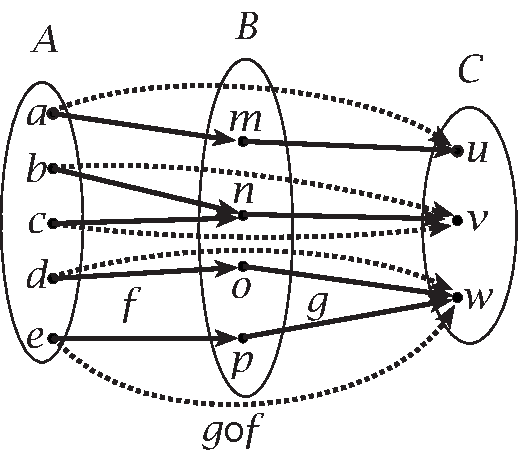
\includegraphics[scale=0.55]{images/arrowcompose.pdf}
\caption{Arrows for the composition $g \circ f$ are dotted.}
\label{arrowcomposefig}
\end{figure}
%\end{center}
Notice how we write the result as $g \compose f$ with $g$ on the left and $f$ on the right even though $f$ appears on the left in Figure~\ref{arrowcomposefig}. This is an unfortunate consequence of the fact that when we calculate $g \bigl(f(x) \bigr)$ we work right to left, computing $f(x)$ first and applying $g$ to the result.
\end{example}

Note that in the definition of $g \compose f$ (Definition~\ref{defn:composition}), the domain of~$g:B\rightarrow C$ is required to be equal to the codomain of~$f:A \rightarrow B$. Actually $g \compose f$ can be defined as long as the domain of $g$ \emph{contains} the specified codomain of~$f$. This is true because the codomain of a function is not unique: if $f: A \rightarrow D$ and $D \subset B$, then $B$ is also a valid codomain of $f$. The reason for the requirement on the domain of $g$ is further explored in the following exercise.

\begin{exercise}\label{exercise:functions:ComposeDomainMatch}
Let $f \colon \mathbb{N} \to \mathbb{Z}_5$ defined by 
$f(n) \equiv  n \pmod{5}$.
\noindent
Let $g \colon \mathbb{R} \to \mathbb{R}$ defined by:
$$g(x) = x^2.$$

\begin{enumerate}[(a)]
\item
Is it possible to define $f \compose g$? \emph{Explain} your answer.
\item
Is it possible to define $g \compose f$? \emph{Explain} your answer.
\end{enumerate}
\end{exercise}

\begin{exercise}\label{exercise:functions:ComposeExers-form} 
 The formulas define functions $f$ and~$g$ from~$\mathbb{R}$ to~$\mathbb{R}$. Find formulas for $(f \compose g)(x)$ and $(g \compose f)(x)$.
\begin{enumerate}[(a)]
\item \label{ComposeExers-form-(3x+1)(x2+2)}
 $f(x) = 3x + 1$ and $g(x) = x^2 + 2$ 
\item \label{ComposeExers-form-(3x+1)(x-1/3)}
 $f(x) = 3x + 1$ and $g(x) = (x-1)/3$ 
\item \label{ComposeExers-form-(ax+b)(cx+d)}
 $f(x) = ax + b$ and $g(x) = c x + d$ (where $a,b,c,d \in \real$)
\item \label{ComposeExers-form-(|x|)(x2)}
 $f(x) = |x|$ and $g(x) = x^2$ 
\item \label{ComposeExers-form-(|x|)(-x)}
 $f(x) = |x|$ and $g(x) = -x$ 
\end{enumerate}
\end{exercise}

\begin{exercise}\label{exercise:functions:ComposeExers-pairs} 
 Let $A = \{1,2,3,4\}$, $B = \{\var{a},\var{b},\var{c},\var{d}\}$, and $C = \{\clubsuit, \diamondsuit, \heartsuit, \spadesuit\}$. The sets of ordered pairs in each part are functions $f \colon A \to B$ and $g \colon B \to C$. Represent $g \compose f$ as a set of ordered pairs.
\smallskip
\begin{enumerate}[(a)]
\item \label{ComposeExers-pairs-(abcd)(cdhs)} 
 $f = \{(1,\var{a}), (2,\var{b}), (3,\var{c}), (4,\var{d})\}$,
 \\ $g = \{(\var{a},\clubsuit), (\var{b},\diamondsuit), (\var{c},\heartsuit), (\var{d},\spadesuit) \}$
\smallskip
\item \label{ComposeExers-pairs-(abcd)(cccc)} 
 $f = \{(1,\var{a}), (2,\var{b}), (3,\var{c}), (4,\var{d})\}$,
 \\ $g = \{(\var{a},\clubsuit), (\var{b},\clubsuit), (\var{c},\clubsuit), (\var{d},\clubsuit) \}$
\smallskip
\item \label{ComposeExers-pairs-(bcda)(cshd)} 
 $f = \{(1,\var{b}), (2,\var{c}), (3,\var{d}), (4,\var{a})\}$,
 \\ $g = \{(\var{a},\clubsuit), (\var{b}, \spadesuit), (\var{c},\heartsuit), (\var{d}, \diamondsuit) \}$
\smallskip
\item \label{ComposeExers-pairs-(abcd)(cchs)} 
 $f = \{(1,\var{a}), (2,\var{b}), (3,\var{c}), (4,\var{d})\}$,
 \\ $g= \{(\var{a},\clubsuit), (\var{b},\clubsuit), (\var{c}, \heartsuit), (\var{d}, \spadesuit) \}$
\smallskip
\item \label{ComposeExers-pairs-(abab)(cchs)} 
 $f = \{(1,\var{a}), (2,\var{b}), (3,\var{a}), (4,\var{b})\}$,
 \\ $g = \{(\var{a},\clubsuit), (\var{b},\clubsuit), (\var{c}, \heartsuit), (\var{d}, \spadesuit) \}$
%\item $f = \{(1,\var{a}), (2,\var{b}), (3,\var{c}), (4,\var{d})\}$,
% \\ $g = \{(\var{a},\heartsuit), (\var{b},\clubsuit), (\var{c},\heartsuit), (\var{d},\heartsuit) \}$
\end{enumerate}
\end{exercise}


\subsection*{Proofs involving function composition}

The properties of $f \compose g$ depend on the properties of $f$ and $g$, and vice versa. Usually these properties are proven by using the definition of composition, along with the definitions of other functional properties.  Here is one example.

\begin{example}\label{example:functions:ComposeExers-11}
Suppose $f\colon A \to B$ and $g \colon B \to C$. Show that if 
$$\mbox{$(g \compose f)(a) = a$, for every $a \in A$,} $$
 then $f$ is one-to-one.
 
 \begin{scratchwork}
 We want to show that $f$ is one-to-one; that is if $f(a_1) = f(a_2)$, then $a_1 = a_2$.  We are given that $(g \compose f)(a) = a$, for every $a \in A$.  Therefore for our proof we should assume $f(a_1) = f(a_2)$, and use the given statement to somehow get to $a_1 = a_2$. 
 \end{scratchwork}
 
 \begin{proof}
Given that $(g \compose f)(a) = a$, for every $a \in A$, by the definition of composition, this means
that, for any $a_1, a_2 \in A$ we have
$$ g \bigl( f(a_1) \bigr) = a_1 \mbox{ and }  g \bigl( f(a_2) \bigr) = a_2.$$
Now suppose $f(a_1) = f(a_2)$. Then by the definition of a function, 
$$ g \bigl( f(a_1) \bigr) =  g \bigl( f(a_2) \bigr)$$
By our original hypothesis we then get $a_1 = a_2$, and thus $f$ is one-to-one.
\end{proof}    
 \end{example}

\begin{example}\label{example:functions:CompositionTheoryExers-gofonto} 
 Suppose $f \colon A \to B$ and $g \colon B \to C$. Show that if $f$ and~$g$ are onto, then $g \compose f$ is onto.

 \begin{proof}
Let $c$ be an arbitrary  element of $C$. Since $g$ is onto, there exists a $b$ in  $B$ such that $g(b) = c$.  Since $f$ is onto, there exists a $a$ in  $A$ such that $f(a) = b$. It follows that  $g \compose f(a) = g(f(a)) = g(b) = c$. Since $c$ is an arbitrary element of $C$, this implies that $g \compose f$ is onto.
\end{proof}    
 \end{example}


\begin{example}\label{example:functions:CompositionTheoryExers-g11} 
Suppose $f \colon A \to B$ and $g \colon B \to C$. Show that if $g \compose f$ is one-to-one, 
 and the range of~$f$ is~$B$, then $g$ is one-to-one. 

 \begin{proof}
Suppose $b_1$ and $b_2$ are distinct elements of $B$.  Since the range of $f$ is $B$, it follows that there exist $a_1 \neq a_2$ such that $f(a_1) = b_1$ and $f(a_2) = b_2$.  Since $g \compose f$ is one-to-one, it follows that $g \compose f(a_1) \neq g \compose f(a_2)$. But by definition of $\compose$, $g \compose f(a_1) = g(f(a_1)) = g(b_1)$; and similarly $g \compose f(a_2) =  g(b_2)$. By substitution, it follows that  $g(b_1) \neq g(b_2)$. Thus distinct elements of $B$ always map to distinct elements of $C$ under the function $g$: which is the same as saying that $g$ is one-to-one. 

An alternative proof runs as follows. Let $c \in C$ be such that $c =g(b_1)$  and $c= g(b_2)$. Then since the range of $f$ is B, there exist $a_1$ and  $a_2$ such that $f(a_1) = b_1$ and $f(a_2) = b_2$. It follows  by substitution that  $g(f(a_1)) = g(f(a_2))$. But this is the same as saying that $g \compose f(a_1) = g \compose f(a_2)$. Since  $g \compose f$ is one-to-one, it follows that $a_1 = a_2$. Applying $f$ to both sides of this equation gives $f(a_1) = f(a_2)$, or $b_1 = b_2$. We have shown that  for any $c \in  C$, there is at most one $b \in B$ such that $g(b) = c$. This means that $g$ is one-to-one.
\end{proof}    
 \end{example}

\begin{exercise}\label{exercise:functions:CompositionTheoryExers} \ 
\begin{enumerate}[(a)]
 \item \label{CompositionTheoryExers-gof11} 
 Suppose $f \colon A \to B$ and $g \colon B \to C$. Show that if $f$ and~$g$ are one-to-one, then $g \compose f$ is one-to-one. 
  \item \label{CompositionTheoryExers-f11} 
Suppose $f \colon A \to B$ and $g \colon B \to C$. Show that if $g \compose f$ is one-to-one, then $f$ is one-to-one.
 \item \label{CompositionTheoryExers-gonto} 
Suppose $f \colon A \to B$ and $g \colon B \to C$. Show that if $g \compose f$ is onto, then $g$ is onto.
 \item \label{CompositionTheoryExers-egNotOnto} 
Give an example of functions $f \colon A \to B$ and $g \colon B \to C$, such that $g \compose f$ is onto, but $f$ is not onto. 
% (\emph{Hint}: Let $A = B = \real$, $C = [0,\infty)$ and $f(x) = x^2$. Find a $g$ that works, and verify your example.)
 \item \label{CompositionTheoryExers-fonto} 
Suppose $f \colon A \to B$ and $g \colon B \to C$. Show that if $g \compose f$ is onto, 
 and $g$~is one-to-one, then $f$ is onto.
 \item  \label{CompositionTheoryExers-gNot11} 
Define $f \colon [0,\infty) \to \real$ by $f(x) = x$. Find a function $g \colon \mathbb{R} \to \mathbb{R}$ such that 
$g \compose f$ is one-to-one, but $g$ is \emph{not} one-to-one.
% and $g \colon \mathbb{R} \to \mathbb{R}$ by $g(x) = |x|$. Show that $g \compose f$ is one-to-one, but $g$ is \emph{not} one-to-one.
 \item  \label{CompositionTheoryExers-what} 
Suppose $f$ and~$g$ are functions from~$A$ to~$A$. If $f(a) = a$ for every $a \in A$, then what are $f \compose g$ and $g \compose f$?
\end{enumerate}
\end{exercise}
 
The preceding exercises and examples can be used to prove the following:

 \begin{exercise}\label{exercise:functions:BijectionComposeExer}
 Suppose $f \colon A \to B$ and $g \colon B \to C$.
 \begin{enumerate}[(a)]
 \item \label{BijectionComposeExer-gf}
 Show that if $f$ and~$g$ are bijections, then $g \compose f$ is a bijection. (\emph{Hint}: You just need to show that $g \compose f$ is both one-to-one and onto. Use the previous exercises.)
 \item  \label{BijectionComposeExer-g}
Show that if $f$ and $g\compose f$ are bijections, then $g$ is a bijection.
 \item \label{BijectionComposeExer-f}
Show that if $g$ and~$g \compose f$ are bijections, then $f$ is a bijection.
 \end{enumerate}
 \end{exercise}
 
 

 \begin{exercise}\label{exercise:functions:InverseMakesBijectionExer}
 Suppose 
 \begin{itemize}
 \item $f \colon A \to B$,
 \item  $g \colon B \to A$,
 \item $(g \compose f)(a) = a$, for every $a \in A$,
 and
 \item $(f \compose g)(b) = b$, for every $b \in B$.
 \end{itemize}
 Show that $f$ is a bijection.
 \end{exercise}
  

%\begin{summary}
%\item Important definitions:
%\begin{itemize}
%\item composition of functions
%\end{itemize}
%\item Notation:
%\begin{itemize}
%\item composition $(g \compose f) (x)= g\bigl(f(x)\bigr)$
%\end{itemize}
%\end{summary}


 
 \section{Inverse Functions}

%\begin{quote}
%\it Backwards poets write inverse.
%\newline
%\small\rm\sf
%\hbox{ }\hfil 
%Author unknown\break
%\end{quote}

\subsection*{Concept and Definition}

\medskip\noindent
The word "inverse" commonly means something that is ``backwards'' or ``opposite'' to something else.  So an inverse of a function should be  a function that is somehow backwards or opposite to the original  function.  
You have actually seen inverse functions many times before, perhaps without realizing it.
%All students of mathematics have experience with solving an equation for~$x$, and in doing so you might have seen an example of inverse functions.

\begin{example}
In Example~\ref{example:functions:5x-7BijectionEg}, it was shown that $f(x) = 5x - 7$ is a bijection. A quick look at the proof reveals that the formula
$$x =  \frac{y+7}{5} $$
plays a key role.  This formula is obtained by replacing $f(x)$ in $f(x) = 5x - 7$ with $y$, and solving for $x$.

In order to see $x = \frac{y+7}{5}$ as an ``inverse function," we translate into the language of functions, by defining $g \colon \mathbb{R} \to \mathbb{R}$  by $g(y) = (y+7)/5$. Then the above assertion can be restated as:
\begin{align*} \label{y=f(x)<>x=g(y)}
 y = f(x) \qquad \eiff \qquad x = g(y) .
 \end{align*}
This tells us that $g$ does exactly the opposite of what~$f$ does: if $f$ takes $x$ to~$y$, then $g$ takes $y$ to~$x$. We will say that $g$ is an ``inverse" of~$f$.
\end{example}


The following proof provides a restatement of this result that will be used in the official definition of inverse functions. I will prove part (a); you will prove part (b).

 \begin{example}\label{example:functions:xgyInverseExer}
 Suppose  that $f \colon X \to Y$
 and $g \colon Y \to X$, such that
 $$ \forall x \in X, \forall y \in Y, \bigl(y = f(x) \eiff x = g(y) \bigr). $$
Then the following statements are also true:
  \begin{enumerate} \renewcommand{\theenumi}{\alph{enumi}}
 \item  \label{x=g(y)->InverseExer-f(g(y))}
 $f \bigl( g(y) \bigr) = y$ for all $y \in Y$,
 and
 \item  \label{x=g(y)->InverseExer-g(f(x))}
 $g \bigl( f(x) \bigr) = x$ for all $x \in X$.
 \end{enumerate}

 
 \begin{proof}
 \begin{enumerate}[(a)]
 \item
For any $y \in Y$, from the above statement we know two things:  
$$\exists x \in X \mbox{ s.t. } g(y) = x$$ 
and
$$\mbox{ for that particular } x, f(x) = y$$
Therefore, 
$$f \bigl( g(y) \bigr) = f(x) = y, \forall y \in Y$$
\end{enumerate}
\end{proof}

\begin{exercise}
Prove part (b) of Example~\ref{example:functions:xgyInverseExer}
\end{exercise}
 \end{example}

Finally, we can give the definition of an inverse function:\index{Function!inverse functions}\index{Inverse!of a function}\index{Inverse function!definition of}

 \begin{defn}\label{def:invfna}
 Suppose 
 \begin{itemize}
 \item $f \colon X \to Y$,
 and
 \item $g \colon Y \to X$,
\end{itemize}
We say that $g$ is an \bfii{ inverse} of~$f$ if and only if:
 \begin{enumerate} \renewcommand{\theenumi}{\alph{enumi}}
 \item $f \bigl( g(y) \bigr) = y$ for all $y \in Y$,
 and
 \item $g \bigl( f(x) \bigr) = x$ for all $x \in X$.
 \end{enumerate}
 \end{defn}
 

 \begin{example}
The husband of the wife of any married man is the man himself -- in other words,
$$ \var{husband}\bigl( \var{wife} (y) \bigr) = y. $$
Also, the wife of the husband of any married woman is the woman herself, so that
$$ \var{wife}\bigl( \var{husband} (x) \bigr) = x . $$
It follows that
the $\var{wife}$ function is an inverse of the~$\var{husband}$ function. In fact, it's pretty clear that $\var{husband}$ is the \emph{only} inverse of $\var{wife}$.
\end{example}
 

 \begin{exercise}\label{exercise:functions:VerifyInverseExers}
 In each case, use Definition~\ref{def:invfna} to determine whether $g$ is an inverse of~$f$.
 \begin{enumerate}[(a)]
 \item \label{VerifyInverseExers-(9x-6)}
$f \colon \real \to \real$ is defined by $f(x) = 9x - 6$ and 
 \\ $g \colon \real \to \real$ is defined by $g(x) = (x + 6)/9$.
 \item \label{VerifyInverseExers-(x^2)}
$f \colon \real^+ \to \real^+$ is defined by $f(x) =2x^2$ and 
 \\ $g \colon \real^+ \to \real^+$ is defined by $g(x) = \sqrt{x}/2$.
 \item \label{VerifyInverseExers-(1/x)}
$f \colon \real^+ \to \real^+$ is defined by $f(x) = 2/x$ and 
 \\ $g \colon \real^+ \to \real^+$ is defined by $g(x) = 2/x$.
 \item \label{VerifyInverseExers-(sqrt(x+1)-1)}
$f \colon \real^+ \to \real^+$ is defined by $f(x) = \sqrt{x+1} - 1$ and 
 \\ $g \colon \real^+ \to \real^+$ is defined by $g(x) = x^2 + 2x$.
 \end{enumerate}
 \end{exercise}
   
\subsection*{Which functions have inverses?}

It turns out that most functions do \emph{not} have an inverse.  

\begin{exercise}
Which of the functions depicted  in Figure~\ref{arrowontofig} have inverses?
 \end{exercise}

From the previous exercise, you may have guessed the following rule:

 \begin{thm} \label{InverseBijection}
 Suppose $f\colon X \to Y$. Then $f$ has an inverse $g \colon Y \to X$ if and only if $f$ is a bijection.\index{Function!as a bijection}\index{Bijection!relation to inverse functions}\index{Inverse function!relation to bijection}
 \end{thm}
 
 This is another ``if and only if" proof, so it must be proved in both directions. We will prove the forward direction of this proposition.  You will prove the reverse direction.
 
 \begin{scratchwork}
 The forward direction of Proposition~\ref{InverseBijection} says that if $f \colon X \to Y$ has an inverse $g \colon Y \to X$, then $f$ is a bijection.  In other words we must assume the first statement, and from that prove that $f$ is one-to-one and onto.
 \end{scratchwork}
 
 \begin{proof} \emph{(forward direction)}
 Assume there is a function $g \colon Y \to X$ that is an inverse of~$f$. Then by the definition of an inverse function,
\begin{enumerate}[(a)]
\item $f \bigl( g(y) \bigr) = y$ for all $y \in Y$, and
\item $g \bigl( f(x) \bigr) = x$ for all $x \in X$.
\end{enumerate}
Suppose then that $f(x_1) = f(x_2)$ for some $x_1, x_2 \in X$.  Then since $g$ is a function we have
$$g \bigl( f(x_1) \bigr) = g \bigl( f(x_2) \bigr)$$
Therefore by (b), $x_1 = x_2$. Hence $f$ is one-to-one.

\noindent
Now suppose $y_1 \in Y$.  Then since $g$ is a function, there exists a unique  $x_1 \in X$ such that $g(y_1) = x_1$.  Substituting into (a) we get
\[f \bigl(x_1) \bigr) = y_1.\]
Therefore $\forall y \in Y, \exists x \in X \mbox{ s.t. } f(x) = y$.  Hence $f$ is onto.
So $f$ is both one-to-one and onto: thus $f$ is a bijection.
 \end{proof}

\begin{exercise}
Prove the reverse direction of Proposition~\ref{InverseBijection}.
\end{exercise}

 \begin{exercise}\label{exercise:functions:InverseUniqueExers} 
 \begin{enumerate}[(a)]
 \item \label{InverseUniqueExers-bij}
 Prove that any inverse of a bijection is a bijection.
 \item \label{InverseUniqueExers-unique}
 Show that the inverse of a function is \emph{unique}: if $g_1$ and~$g_2$ are inverses of~$f$, then $g_1 = g_2$. 
 \end{enumerate}
 \end{exercise}

\begin{rem}
\begin{enumerate}[(a)]
\item
Exercise~\ref{exercise:functions:InverseUniqueExers} is key because it enables us to talk about \emph{the} inverse of a function, since there is at most one. We will use the special notation $f^{-1}$\index{Inverse function!notation} to denote the inverse of the function $f$.
\item
If $f$ is a function that has an inverse, then it is easy to find~$f^{-1}$ as a set of ordered pairs. Namely, 
$$ f^{-1} = \{\, (y,x) \mid (x,y) \in f \,\} .$$
This is simply a restatement of the fact that
 $$y = f(x) \eiff x = f^{-1}(y) .$$
\end{enumerate}
\end{rem}

\begin{defn}{}
For any set~$A$, define the \terminology{identity map} $\Id_A \colon A \to A$ by $\Id_A(a) = a$ for every $a \in A$.
\end{defn}\index{Identity map} 

\begin{exercise}
\begin{enumerate}[(a)]
\item
Show that $\Id_A$ is invertible
\item
Find the inverse of $\Id_A$
\end{enumerate}
\end{exercise}

\begin{exercise}\label{exercise:functions:InverseIdentityExers}\ 
\begin{enumerate}[(a)]
\item \label{InverseIdentityExers-InvOfComp}
Suppose $f \colon A \to B$ and $g \colon B \to C$ are bijections. Show that $(g \compose f)^{-1} = f^{-1} \compose g^{-1}$.
\item \label{InverseIdentityExers-Comp=Id}
Suppose $f \colon X \to Y$ and $g \colon Y \to X$. Show that $g$ is the inverse of~$f$ if and only if
$$ \mbox{$f \compose g = \Id_Y$ \quad and \quad $g \compose f = \Id_X$} .$$
\item \label{InverseIdentityExers-InvOfInv}
Suppose $f \colon X \to Y$ is a bijection. Show that the inverse of~$f^{-1}$ is~$f$. That is, $(f^{-1})^{-1} = f$.
\end{enumerate}
\end{exercise}

% CPT put this back in if we put in pre-image section
%\begin{warn}
%We have already introduced $f^{-1}$ as notation for pre-images, even when $f^{-1}$ was not a function (that is, even when $f$ was not a bijection).  Be aware that this notation is used in both contexts.
%end{warn}
%
%\begin{summary}
%\item Important definitions:
%\begin{itemize}
%\item inverse function
%\item identity map
%\end{itemize}
%\item A function $f$ has an inverse iff $f$ is a bijection.
%\item Notation:
%\begin{itemize}
%\item $f^{-1}$
%\item $\Id_A \colon A \to A$
%\end{itemize}
%\end{summary}